\documentclass[11pt]{article}

\hoffset        2mm 
\voffset        -15mm
\oddsidemargin  0mm
\topmargin      0.30in
\textwidth      6.25in
\textheight     9in

\usepackage[parfill]{parskip}
\usepackage{graphicx}
\usepackage{amsmath}
%\usepackage{mathtools}
\usepackage{booktabs}
\usepackage{enumerate}
\usepackage{listings}
\usepackage{float}
\usepackage{bigints}
\usepackage{caption}
\usepackage{subcaption}
\usepackage{afterpage}
\usepackage{epstopdf}
\usepackage{commath}
\usepackage{amssymb}

\begin{document}


\begin{center}
{\Large Higher-Order DGFEM Transport Calculations on Polytope Meshes for Massively-Parallel Architectures}\\[8mm]
{Michael W. Hackemack} \\[2mm]
{\em \small Department of Nuclear Engineering, Texas A\&M University, College Station, TX 77843, USA} \\[1mm]
{\em mike\_hack@tamu.edu} \\[6mm]
\end{center}

%%%%%%%%%%%%%%%%%%%%%%%%%%%%%%%%%%%%%%%%%%%%%%%%%%%%%%%%%%%%%%%%%%%%%%
%%%%%%%%%%%%%%%%%%%%%%%%%%%%%%%%%%%%%%%%%%%%%%%%%%%%%%%%%%%%%%%%%%%%%%
\section{Introduction}
\label{sec::intro}

The discontinuous galerkin finite element method (DGFEM) has been widely used to solve the radiation transport equation using the discrete ordinates ($S_N$) approximation \cite{reed1973triplet}. The standard, multigroup $S_N$ neutral particle transport equation (without the position parameter) for a given direction, $\vec{\Omega}_m$, and energy group, $g$, is given by the following,

\begin{equation}
\label{eq::trans_eq}
\vec{\Omega}_m \cdot \vec{\nabla} \Psi_{m,g} + \sigma_{t,g} \Psi_{m,g} (\vec{\Omega}_m) = \sum_{g'=1}^G \sum_{n=0}^{N_a} \frac{2n+1}{4 \pi} \sum_{k=-n}^{n} \left[ \sigma_{s,n}^{g' \rightarrow g}  \Phi_{n,k,g'} Y_{n,k} (\vec{\Omega}_m) + Q_{n,k,g}  \right] ,
\end{equation}

\noindent where $\sigma_{t,g}$ is the total macroscopic cross section, $\sigma_{s,n}^{g' \rightarrow g}$ are the macroscopic scattering moments, $\Phi_{n,k,g'}$ are the solution spherical harmonic moments, and $Q_{n,k,g}$ are the distributed source moments \cite{lewis1984computational}. 

We next restrict our problem to a single energy group and simplify the right-hand-side sources, lay down a mesh, $\mathbb{T}_h$, over our problem, multiply by a basis function, $b_m$, analyze a single cell, $K$, integrate over the volume of the cell, and apply Gauss' theorem to yield,

\begin{equation}
\label{eq::disc_trans_eq_cellK}
- \left( \vec{\Omega}_m \cdot  \vec{\nabla} b_m, \Psi_{m} \right)_{K} + \sum_{f=1}^{N_f^K} \Big< ( \vec{\Omega}_m \cdot \vec{n}_f ) \, b_m, \tilde{\Psi}_m  \Big>_{f}  + \Big(  \sigma_{t} b_m ,   \Psi_{m} \Big)_{K} = \left(  b_m ,   Q_m \right)_{K}
\end{equation}

\noindent where $\vec{n}_f$ is the outward normal direction for face $f$ on the cell $K$ boundary and $N_f^K$ is the number of faces on cell $K$. The volume and surface inner products have the form,

\begin{equation}
\label{eq::inner_prod}
\Big( u,v \Big)_K \equiv \int_K u \, v \, d \vec{r} \qquad \text{and} \qquad \Big< u,v \Big>_f \equiv \int_f u \, v \, d s ,
\end{equation}

\noindent respectively. The across-cell boundary flux, $\tilde{\Psi}_m$, is boundary dependent. We apply the ubiquitous {\em upwind scheme} 

\begin{equation}
\label{eq::upwind_eqs}
\tilde{\Psi}_m (\vec{r})  = 
\begin{cases}
\Psi_m^{-} , & \partial K^+ \\
\Psi_m^{+}, & \partial K^- \backslash \partial \mathcal{D} \\
\Psi_m^{inc}, & \partial K^- \cap \partial \mathcal{D}^d \\
\Psi_{m'}^{-}, & \partial K^- \cap \partial \mathcal{D}^r
\end{cases}
\end{equation}

\noindent where the trace is defined as: $\Psi_m^{\pm} (\vec{r}) \equiv \lim_{s \rightarrow 0^{\pm}} \Psi_m \Big( \vec{r} + s (\vec{\Omega}_m \cdot \vec{n}) \vec{n} \Big)$. We then insert the upwind notation of Eq. (\ref{eq::upwind_eqs}) into Eq. (\ref{eq::disc_trans_eq_cellK}) to yield the full set of spatially discretized equations for cell $K$,

\begin{equation}
\label{eq::full_cellK_disc}
\begin{aligned}
-  \Big( \vec{\Omega}_m \cdot  & \vec{\nabla} b_m, \Psi_{m} \Big)_{K}   + \Big(  \sigma_{t} b_m ,   \Psi_{m} \Big)_{K} +  \Big< ( \vec{\Omega}_m \cdot \vec{n} ) \, b_m, {\Psi}_m^{-}  \Big>_{\partial K^+}  \\
  + & \Big< ( \vec{\Omega}_m \cdot \vec{n} ) \, b_m, {\Psi}_m^{+}  \Big>_{\partial K^- \backslash \partial \mathcal{D}}  + \Big< ( \vec{\Omega}_m \cdot \vec{n} ) \, b_m, {\Psi}^{-}_{m'}  \Big>_{\partial K^- \cap \partial \mathcal{D}^r}  \\
= & \left(  b_m ,   Q_m \right)_{K} + \Big< ( \vec{\Omega}_m \cdot \vec{n} ) \, b_m, {\Psi}_m^{inc}  \Big>_{\partial K^- \cap \partial \mathcal{D}^d} 
\end{aligned} \, .
\end{equation}

At this point we note that we have not specified a mesh or basis function type. We have simply left them as an unspecified dual. In base finite element theory, the basis functions are collections of polynomial functions with measure on local elements within the domain \cite{ern2013theory}. A particular application of the Bramble-Hilbert lemma states that we can achieve error convergence rates between the true solution,$u$, and the discretized solution, $u_h$, by,

\begin{equation}
\label{eq::bf_conv_rate_h}
|| u - u_h ||_{L_2} = C h^{p+1}
\end{equation}

\noindent where $h$ is the maximum diameter of a mesh element, $p$ is the polynomial order of the basis functions, and $C$ is a constant independent of the mesh \cite{bramble1970estimation}. If $h$ is difficult to estimate for a particular mesh type, we can proportionally relate it to the number of spatial degrees of freedom in the problem: $N_{dof} \propto h^{-d}$, where $d$ is the dimensionality of the problem (1,2,3). Using this relation, Eq. (\ref{eq::bf_conv_rate_h}) can be rewritten to be dependent on the number of spatial degrees of freedom,

\begin{equation}
\label{eq::bf_conv_rate_DOF}
|| u - u_h ||_{L_2} = C N_{dof}^{- \frac{p+1}{d}},
\end{equation}

\noindent where we note that the constants, $C$, in Eqs. (\ref{eq::bf_conv_rate_h}) and (\ref{eq::bf_conv_rate_DOF}) are not the same. We plot the relations of Eqs. (\ref{eq::bf_conv_rate_h}) and (\ref{eq::bf_conv_rate_DOF}) in Figure \ref{fig::conv_rates} for different polynomial orders. We can see from the relationship of mesh cell size and number of spatial degrees of freedom to the error, that using basis functions with higher-order polynomial interpolations leads to improved convergence rates. As long as the number of spatial degrees of freedom does not grow proportionally to the polynomial order, we expect to achieve more accurate solution estimates in relation to the work required to solve the problem with higher-order interpolants.

\begin{figure}[hbt]
\centering
	\begin{subfigure}[b]{0.475\textwidth}
		\centering
		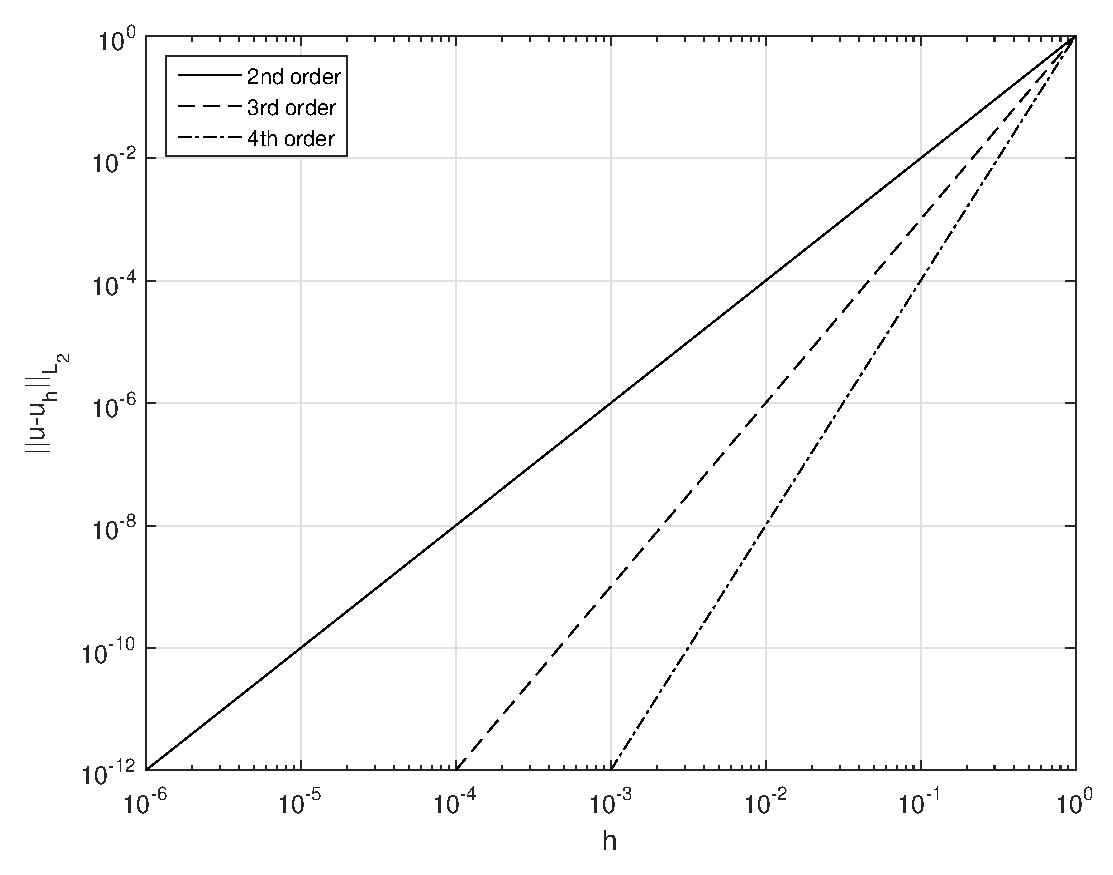
\includegraphics[width=\textwidth]{figures/hconv_larger.eps}
		\caption{}
	\end{subfigure}
	\hfill
	\begin{subfigure}[b]{0.475\textwidth}
		\centering
		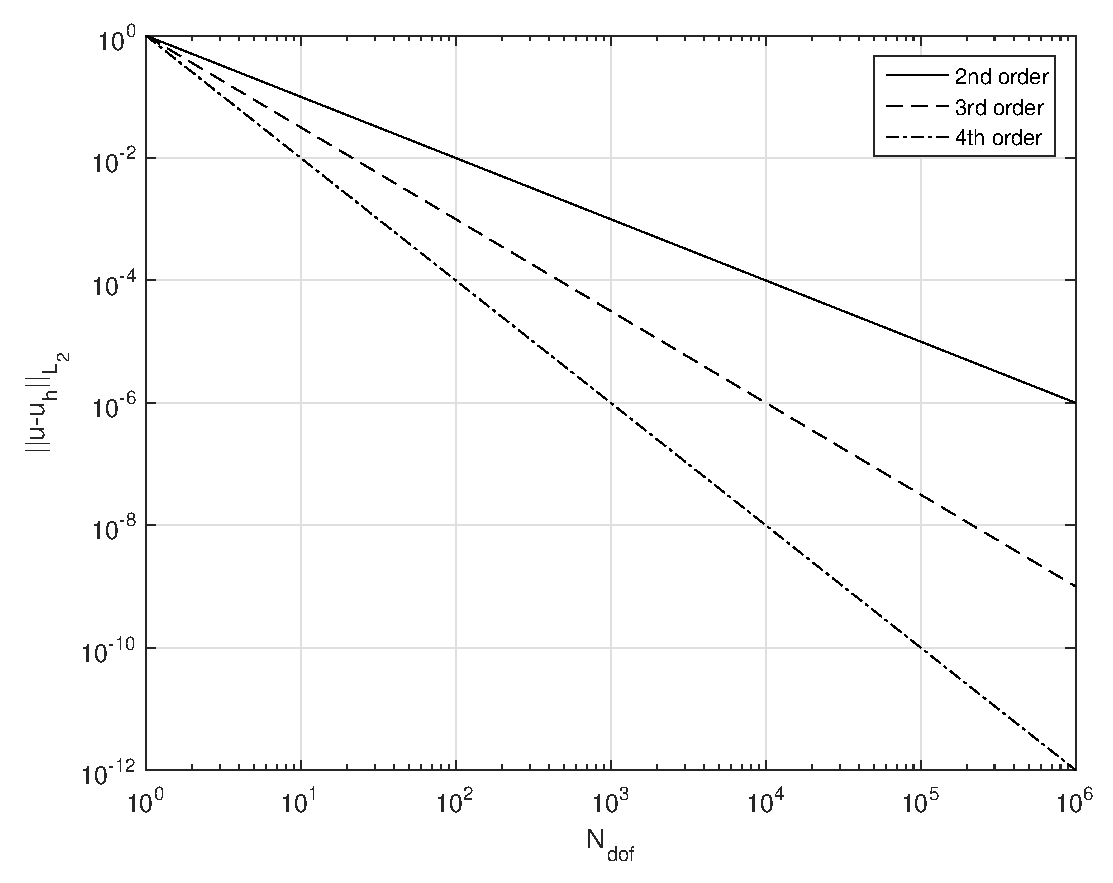
\includegraphics[width=\textwidth]{figures/Nconv_larger.eps}
		\caption{}
	\end{subfigure}
\caption{Theoretical convergence rates of transport solutions with no irregularity based on (a) mesh cell measure and (b) number of spatial degrees of freedom.}
\label{fig::conv_rates}
\end{figure}

For the finite element method, analysis has typically been performed on simple element types: triangles and quadrilaterals in 2D and tetrahedra and hexahedra in 3D \cite{akin1982application}. However, in more recent years there has been a growing interest in different research communities to apply the finite element method to polytope mehes (polygons and polyhedra). Some of the main benefits for using arbitrary polygonal/polyhedral meshes are the following:

\vspace{4mm}
\begin{enumerate}
	\item Polytope mesh cells are now being employed in other physics communities - most notably computational fluid dynamics (CFD)\cite{ref::star_CCM};
	\item They are believed to reduce the number of unknowns to solve with equivalent accuracy;
	\item They can reduce cell/face counts which can reduce algorithm wallclock times depending on the solution method;
	\item They can allow for transition elements between different portions of the domain (e.g., tetrahedral elements bordering hexahedral elements at the border of the boundary layer);
	\item They can easily be split along cut planes - allowing the mesh to be partitioned into regular or irregular divisions as well as be generated by simplical meshing techniques across processor sets in parallel;
	\item Hanging nodes from non-conforming meshes, like those that naturally arise from locally refined/adapted meshes, are no longer necessary. 
\end{enumerate}
\vspace{4mm}

It is because of both these benefits (higher-order FEM basis functions and polytope meshes) which have governed the work going into this dissertation. We seek to analyze and compare different linear polygonal basis functions  for use in DGFEM transport calculations. We then continue this analysis with a quadratic serendipity extension to these linear polygonal basis functions \cite{rand2014quadratic}. We then wish to take the knowledge gained from this polytope DGFEM transport calculation analysis to drive further research into the preconditioning of the DGFEM transport equation for use in massively-parallel computer architectures.

The rest of this proposal is organized as follows. In Section \ref{sec::PS}, we give a brief overview of the existing methodologies used for DGFEM transport. In Section \ref{sec::CW}, we present an overview of the work that has been completed to date. In Section \ref{sec::OW}, we present the remaining work that still needs to be accomplished. Finally, Section \ref{sec::ER} provides a summary of all the expected results that is to be completed with this dissertation work.

%%%%%%%%%%%%%%%%%%%%%%%%%%%%%%%%%%%%%%%%%%%%%%%%%%%%%%%%%%%%%%%%%%%%%%
%%%%%%%%%%%%%%%%%%%%%%%%%%%%%%%%%%%%%%%%%%%%%%%%%%%%%%%%%%%%%%%%%%%%%%
\section{Existing Methodology}
\label{sec::PS}
% Transport and FEM Portion

% DSA Portion
The ability to efficiently invert the transport (streaming and collision) operator does not necessarily mean that transport solutions can be easily obtained. In general, radiation transport solutions are obtained iteratively. The simplest and widely-used method is a fixed-point scheme ({\em i.e.} richardson iteration) ubiquitously called source iteration (SI) in the transport community. Unfortunately, the iteration process of SI can converge arbitrarily slowly if the problem is optically thick \cite{ref::adams_larsen_iter_methods}. This corresponds to long mean free paths for neutronics problems. This also corresponds to time steps and material heat capacities tending to infinity and zero, respectively, for thermal radiative transport (TRT) problems.

For these problem regimes in which solution is prohibitively slow, additional steps should be taken to speed up, or accelerate, solution convergence \cite{ref::adams_larsen_iter_methods}. The most used methods to assist in solution convergence are often called synthetic acceleration techniques. These techniques were first introduced by Kopp  \cite{kopp1963synthetic} and Lebedev \cite{lebedevI,lebedevII,lebedevIII,lebedevIV,lebedevV,lebedevVI,lebedevVII} in the 1960's. From Kopp's and Lebedev's work, Gelbard and Hageman then introduced two synthetic acceleration options for the low-order operator: diffusion and $S_2$ \cite{gelbard1969synthetic}. Their diffusion preconditioning led to efficient convergence properties on fine spatial meshes. Reed then showed that Gelbard and Hageman's diffusion preconditioning would yield a diverging system for coarse meshes \cite{reed1971effectiveness}. At this point in time, no one knew if an unconditionally efficient acceleration method could be derived.

Then in 1976, Alcouffe proposed a remedy to Gelbard and Reed that he called diffusion synthetic acceleration (DSA) \cite{alcouffe1976stable,alcouffe1977DSA,alcouffe1977diffusion}. He showed that if you derived the diffusion operator consistently with the discretized transport operator, then SI could be accelerated with DSA in an efficient and robust manner. Larsen and McCoy then demonstrated that unconditional stability required that consistency be maintained in both spatial and angular discretization in their four-step procedure \cite{larsen1982unconditionally_I,larsen1982unconditionally_II}. However, Adams and Martin then showed that partially-consistent diffusion discretizations could effectively accelerate DFEM discretizations of the neutron transport equation \cite{ref::dsa_DFEM_adams_martin}. Their modified-four-step procedure (M4S), based on Larsen and McCoy's work, was shown to be unconditionally stable for regular geometries, but divergent for unstructured multi-dimensional meshes \cite{warsa2002fully}. In more recent years, alternate discretizations for the diffusion operator have been applied to unstructured multi-dimensional grids. These include the partially consistent Wareing-Larsen-Adams (WLA) DSA \cite{ref::WLA_DSA}, the fully consistent DSA (FCDSA) \cite{warsa2002fully}, and the partially consistent MIP DSA \cite{ref::DSA_wang_ragusa,wang2009adaptive,turcksin2014discontinuous}.

Most recently, the partially consistent MIP DSA method has been shown to be an unconditionally stable acceleration method for the 2D DFEM transport equation on unstructured meshes. Wang showed that it acted as an effective preconditioner for higher-order DFEM discretizations on triangles \cite{ref::DSA_wang_ragusa,wang2009adaptive}. Turcksin and Ragusa then extended the work to arbitrary polygonal meshes \cite{turcksin2014discontinuous}. The MIP diffusion operator is symmetric positive definite (SPD) and was shown to be efficiently invertible with preconditioned conjugate gradient (PCG) and advanced preconditioners such as algebraic multi-grid (AMG) \cite{turcksin2014discontinuous}.

%%%%%%%%%%%%%%%%%%%%%%%%%%%%%%%%%%%%%%%%%%%%%%%%%%%%%%%%%%%%%%%%%%%%%%
%%%%%%%%%%%%%%%%%%%%%%%%%%%%%%%%%%%%%%%%%%%%%%%%%%%%%%%%%%%%%%%%%%%%%%
\section{Current Work}
\label{sec::CW}

Now that we have defined the current state of the art 

%%%%%%%%%%%%%%%%%%%%%%%%%%%%%%%%%%%%%%%%%%%%%%%%%%%%%%%%%%%%%%%%%%%%%%
\subsection{DGFEM Transport Calculations on Polygonal Meshes}
\label{sec::CW_poly}

\begin{figure}
\label{fig::2D_Linear_Summary_unit_square_basis_functions}
\centering
	\begin{subfigure}[b]{0.275\textwidth}
		\centering
		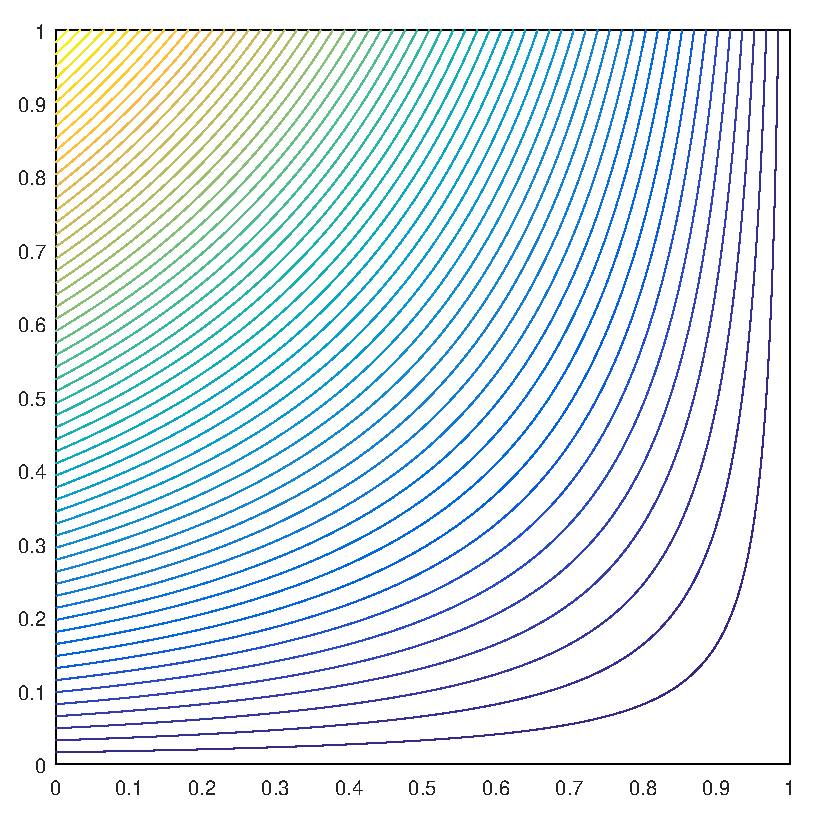
\includegraphics[width=\textwidth]{figures/square_WACHSPRESS1_contour_b4.eps}
		\caption{}
	\end{subfigure}
	\hspace{1cm}
	\begin{subfigure}[b]{0.275\textwidth}
		\centering
		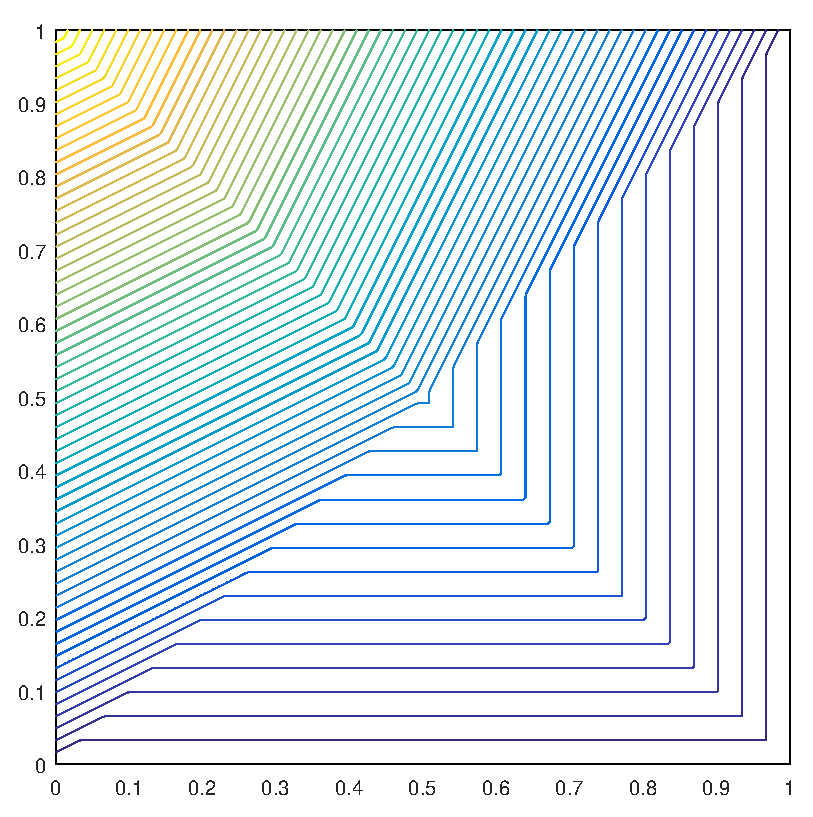
\includegraphics[width=\textwidth]{figures/square_PWLD1_contour_b4.eps}
		\caption{}
	\end{subfigure}
	\vfill
	\begin{subfigure}[b]{0.275\textwidth}
		\centering
		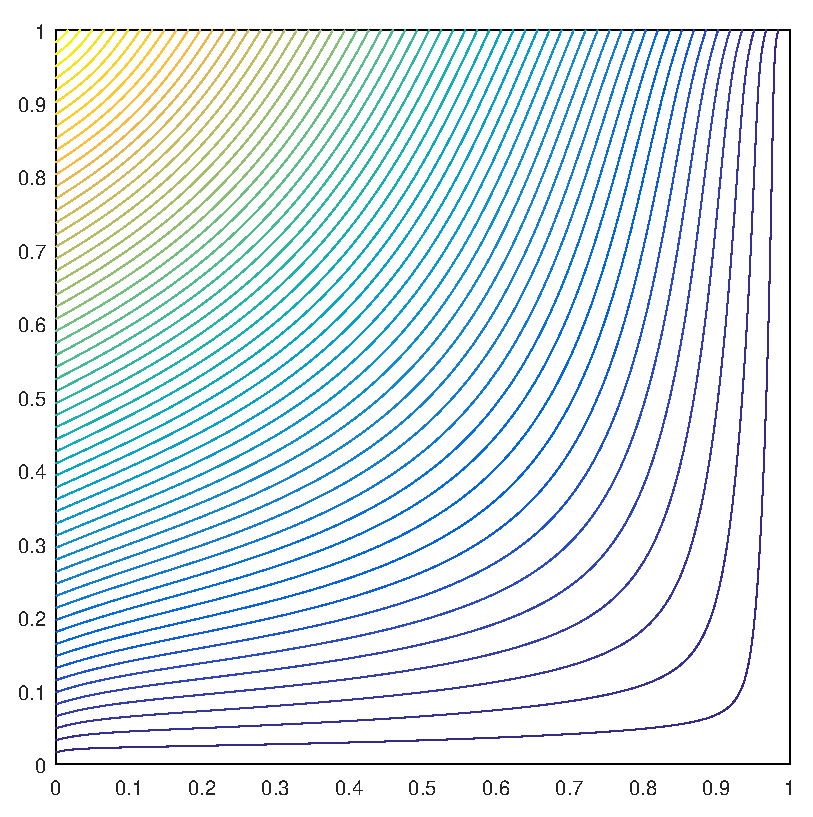
\includegraphics[width=\textwidth]{figures/square_MV1_contour_b4.eps}
		\caption{}
	\end{subfigure}
	\hspace{1cm}
	\begin{subfigure}[b]{0.275\textwidth}
		\centering
		\includegraphics[width=\textwidth]{figures/square_MAXENT1_contour_b4.eps}
		\caption{}
	\end{subfigure}
\caption{Contour plots of the different linear basis functions on the unit square located at vertex (0,1): (a) Wachspress, (b) PWL, (c) mean value, and (d) maximum entropy.}
\end{figure}

\begin{table}[hbt]
\label{tab::lin_poly_summary}
\caption{Summary of the properties of the linear polygonal basis functions used in this work.}
\centering
\begin{tabular}{|c|c|c|c|c|}
\hline
Basis Function & Dimension & Polytope Types & Integration & Direct/Iterative \\
\hline \hline
Wachspress	&2D/3D&	Convex&	Numerical	&Direct\\ \hline
PWL&	1D/2D/3D&	Convex/Concave&	Analytical	&Direct\\ \hline
Mean Value&	2D&	Convex/Concave&	Numerical	&Direct\\ \hline
Max Entropy&	1D/2D/3D	&Convex/Concave&	Numerical&	Iterative\\ \hline
\end{tabular}
\end{table}

The functional interpolation requirements for the linear and quadratic serendipity basis functions for a point $\vec{p}$ are
\iffalse
\begin{equation}
\label{eq::poly_completeness}
\begin{aligned}
\sum_{i=1}^{N}& b_i(\vec{p}) =1 \\
\sum_{i=1}^{N}&  b_i(\vec{p}) \left(  \vec{x}_i - \vec{p}  \right) = \vec{0}
\end{aligned}
\qquad \text{and} \qquad
\begin{aligned}
\sum_{i=1}^{N}& b_i(\vec{p}) =1 \\
\sum_{i=1}^{N}&  b_i(\vec{p}) \left(  \vec{x}_i - \vec{p}  \right) = \vec{0} \\
\sum_{i=1}^{N}&  b_i(\vec{p}) \left(  \vec{x}_i - \vec{p}  \right) \otimes \left(  \vec{x}_i - \vec{p}  \right) = \vec{0}
\end{aligned}
\end{equation}
\fi

\noindent respectively, where $\vec{x}_i$ corresponds to the location of the $i$th basis function. For the linear basis functions this corresponds to vertex $i$. For the quadratic serendipity basis, the interpolation functions lie on the vertices and the midpoint of each face.


\begin{figure}[hbt]
\centering
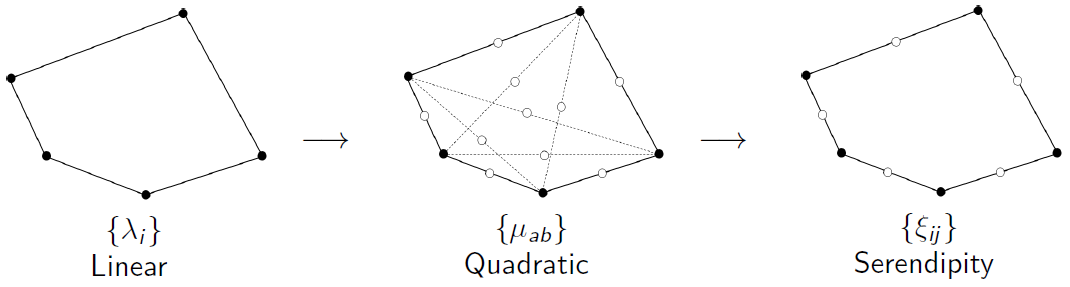
\includegraphics[width=\textwidth]{figures/linear_to_quad_process.png}
\caption{Overview of the process to construct the quadratic serendipity basis functions on polygons. The filled dots correspond to basis functions that maintain the Lagrange property will emply dots do not.}
\label{fig::lin_to_quad_process}
\end{figure}

\begin{figure}
\label{fig::2D_Quadratic_Summary_unit_square_basis_functions_b4}
\centering
	\begin{subfigure}[b]{0.25\textwidth}
		\centering
		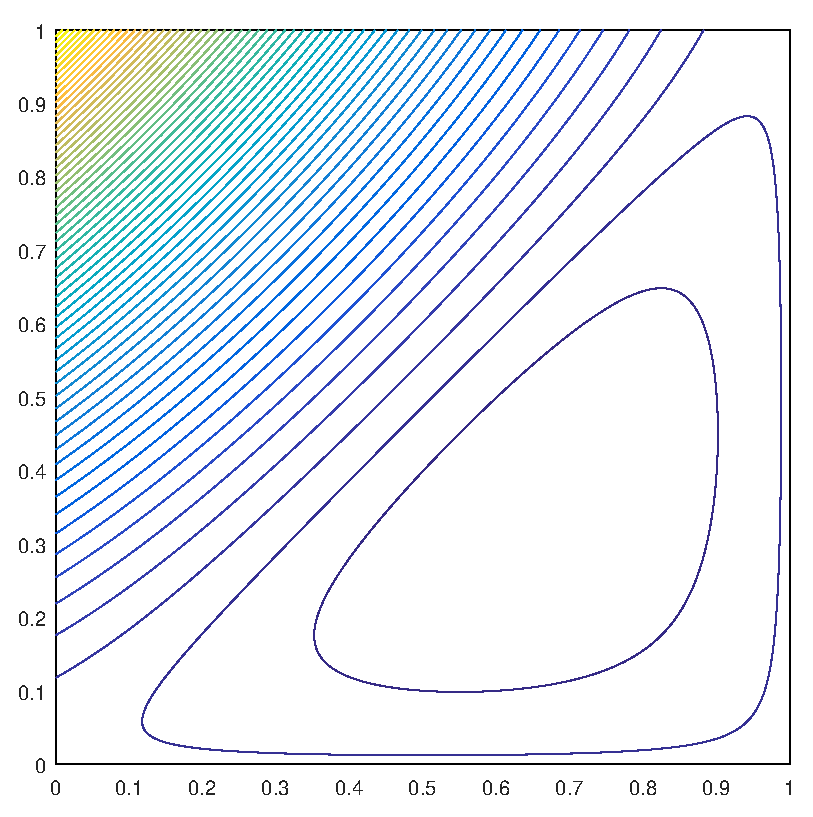
\includegraphics[width=\textwidth]{figures/square_WACHSPRESS2_contour_b4.eps}
		\caption{}
	\end{subfigure}
	\hspace{1cm}
	\begin{subfigure}[b]{0.25\textwidth}
		\centering
		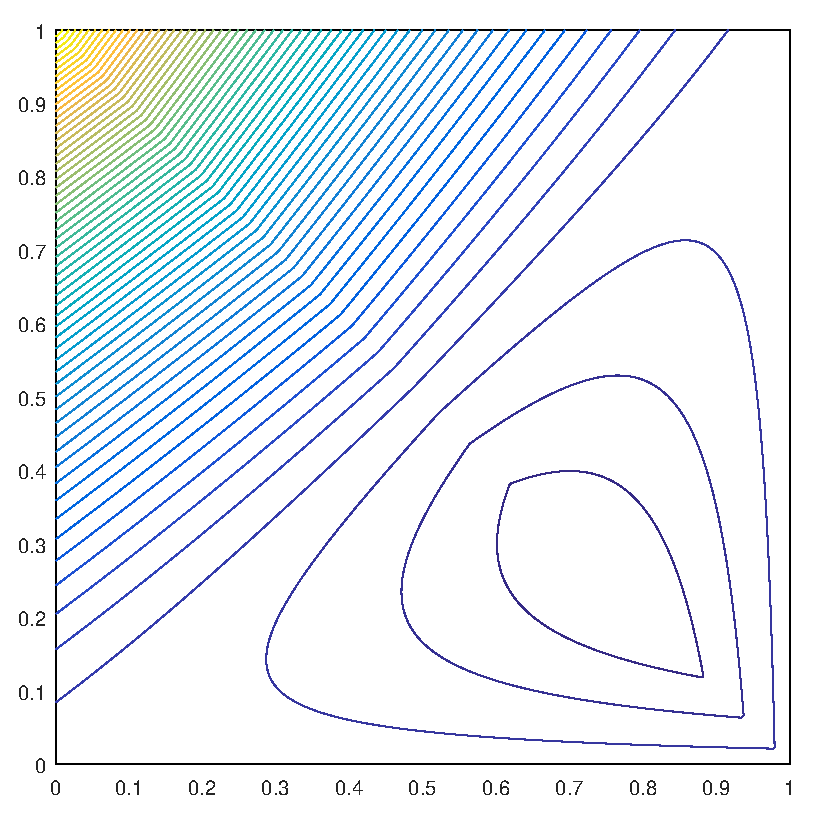
\includegraphics[width=\textwidth]{figures/square_PWLD2_contour_b4.eps}
		\caption{}
	\end{subfigure}
	\vfill
	\begin{subfigure}[b]{0.25\textwidth}
		\centering
		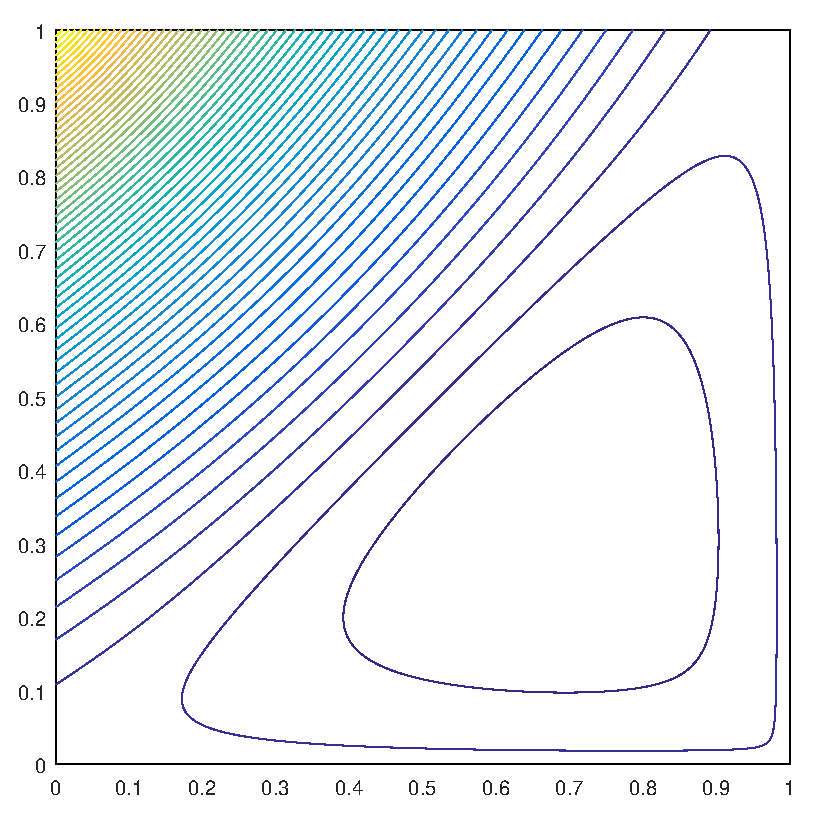
\includegraphics[width=\textwidth]{figures/square_MV2_contour_b4.eps}
		\caption{}
	\end{subfigure}
	\hspace{1cm}
	\begin{subfigure}[b]{0.25\textwidth}
		\centering
		\includegraphics[width=\textwidth]{figures/square_MAXENT2_contour_b4.eps}
		\caption{}
	\end{subfigure}
\caption{Contour plots of the different quadratic serendipity basis functions on the unit square located at vertex (0,1): (a) Wachspress, (b) PWL, (c) mean value, and (d) maximum entropy.}
\end{figure}

\begin{figure}
\label{fig::2D_Quadratic_Summary_unit_square_basis_functions_b8}
\centering
	\begin{subfigure}[b]{0.25\textwidth}
		\centering
		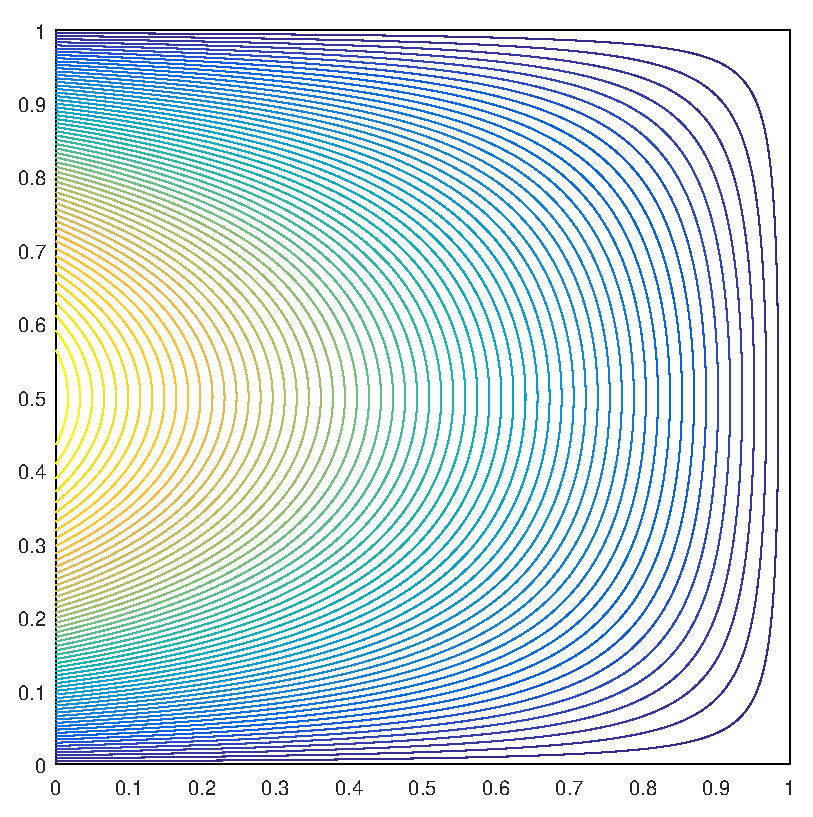
\includegraphics[width=\textwidth]{figures/square_WACHSPRESS2_contour_b8.eps}
		\caption{}
	\end{subfigure}
	\hspace{1cm}
	\begin{subfigure}[b]{0.25\textwidth}
		\centering
		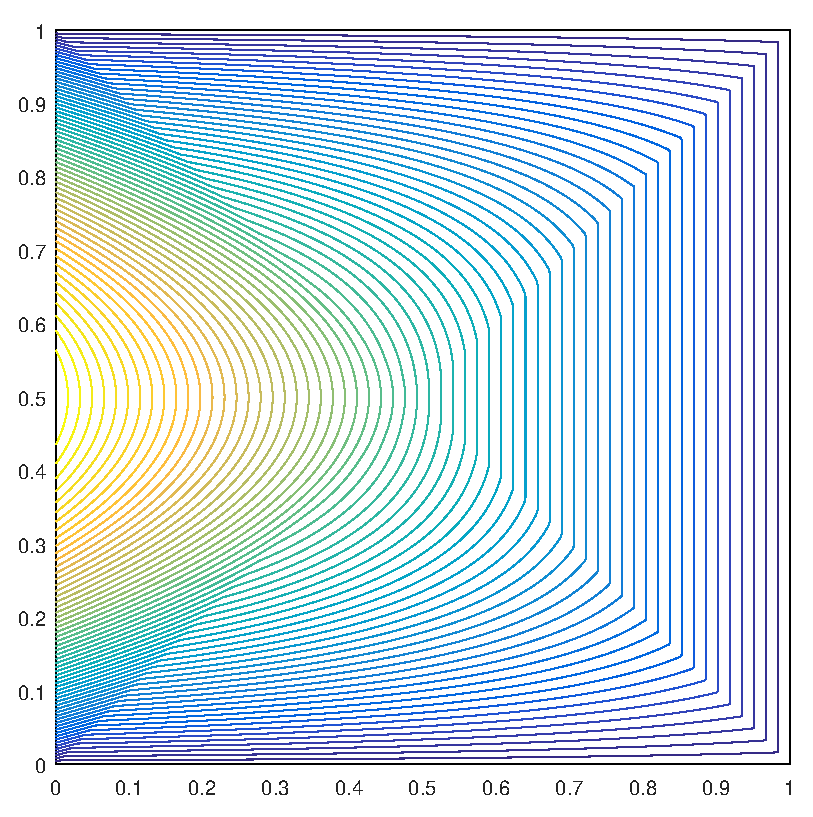
\includegraphics[width=\textwidth]{figures/square_PWLD2_contour_b8.eps}
		\caption{}
	\end{subfigure}
	\vfill
	\begin{subfigure}[b]{0.25\textwidth}
		\centering
		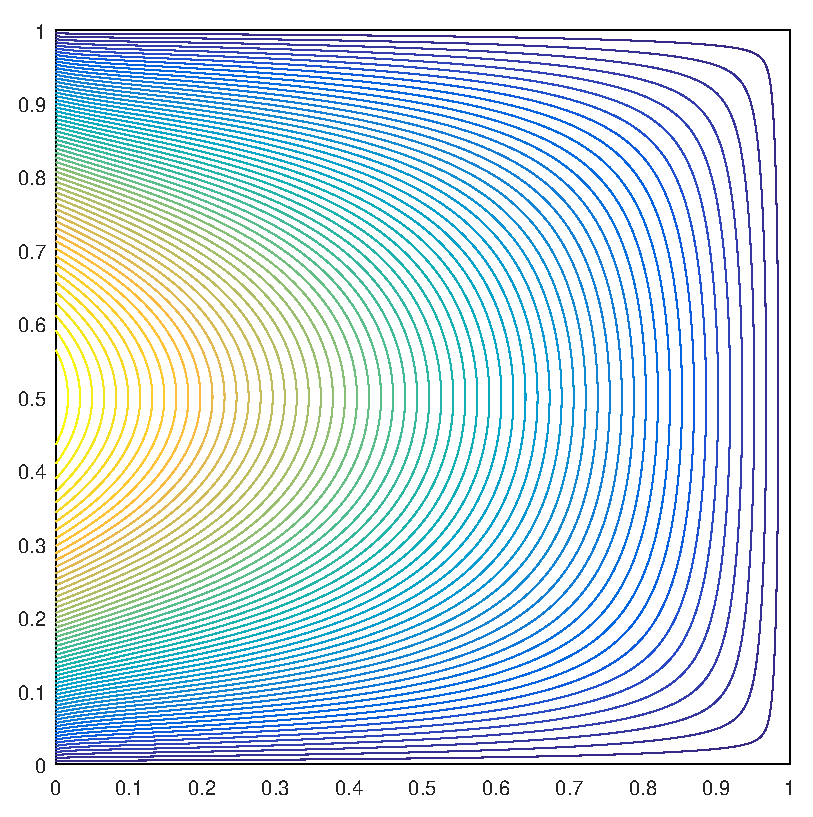
\includegraphics[width=\textwidth]{figures/square_MV2_contour_b8.eps}
		\caption{}
	\end{subfigure}
	\hspace{1cm}
	\begin{subfigure}[b]{0.25\textwidth}
		\centering
		\includegraphics[width=\textwidth]{figures/square_MAXENT2_contour_b8.eps}
		\caption{}
	\end{subfigure}
\caption{Contour plots of the different quadratic serendipity basis functions on the unit square located at vertex (0,1/2): (a) Wachspress, (b) PWL, (c) mean value, and (d) maximum entropy.}
\end{figure}

Having identified the 2D linear polygonal finite element basis functions of interest along with the means to convert them to the quadratic serendipity space, we now wish to analyze their numerical characteristics. First, we wish to verify that all the basis functions can capture an exactly-linear solution on polygonal meshes. We do this by considering the simplified 1-group transport equation,

\begin{equation}
\label{eq::lin_trans_eq}
\mu \frac{\partial  \psi}{\partial x} + \eta \frac{\partial  \psi}{\partial y} + \sigma_t \psi = Q(x,y,\mu,\eta),
\end{equation}

\noindent with the following angular and scalar flux solutions,

\begin{equation}
\label{eq::BF_Results_Linear_fluxsols}
\begin{aligned}
\Psi (x,y,\mu,\eta) &= ax + by + c \mu + d\eta + e,\\
\Phi (x,y) &= 2 \pi \left( ax + by  + e \right).
\end{aligned} 
\end{equation}

\noindent Inserting the angular flux solution of Eq. (\ref{eq::BF_Results_Linear_fluxsols}) into Eq. (\ref{eq::lin_trans_eq}), gives the appropriate functional form for the right-hand-source that yields an exactly-linear solution. Using the level-symmetric quadrature set then guaranties that the linearly-dependent angular terms of the angular flux integrate to 0. We have analyzed all the polygonal basis functions on several different meshes. Figure \ref{fig::lin_sol} presents how the PWL basis functions capture an exactly-linear transport solution on two meshes: a polygonal mesh and a highly-distorted quadrilateral mesh. All the basis functions capture this behavior but we do not present these results for brevity.

\vspace{2mm}
\begin{figure}[hbt]
\centering
	\begin{subfigure}[b]{0.42\textwidth}
		\centering
		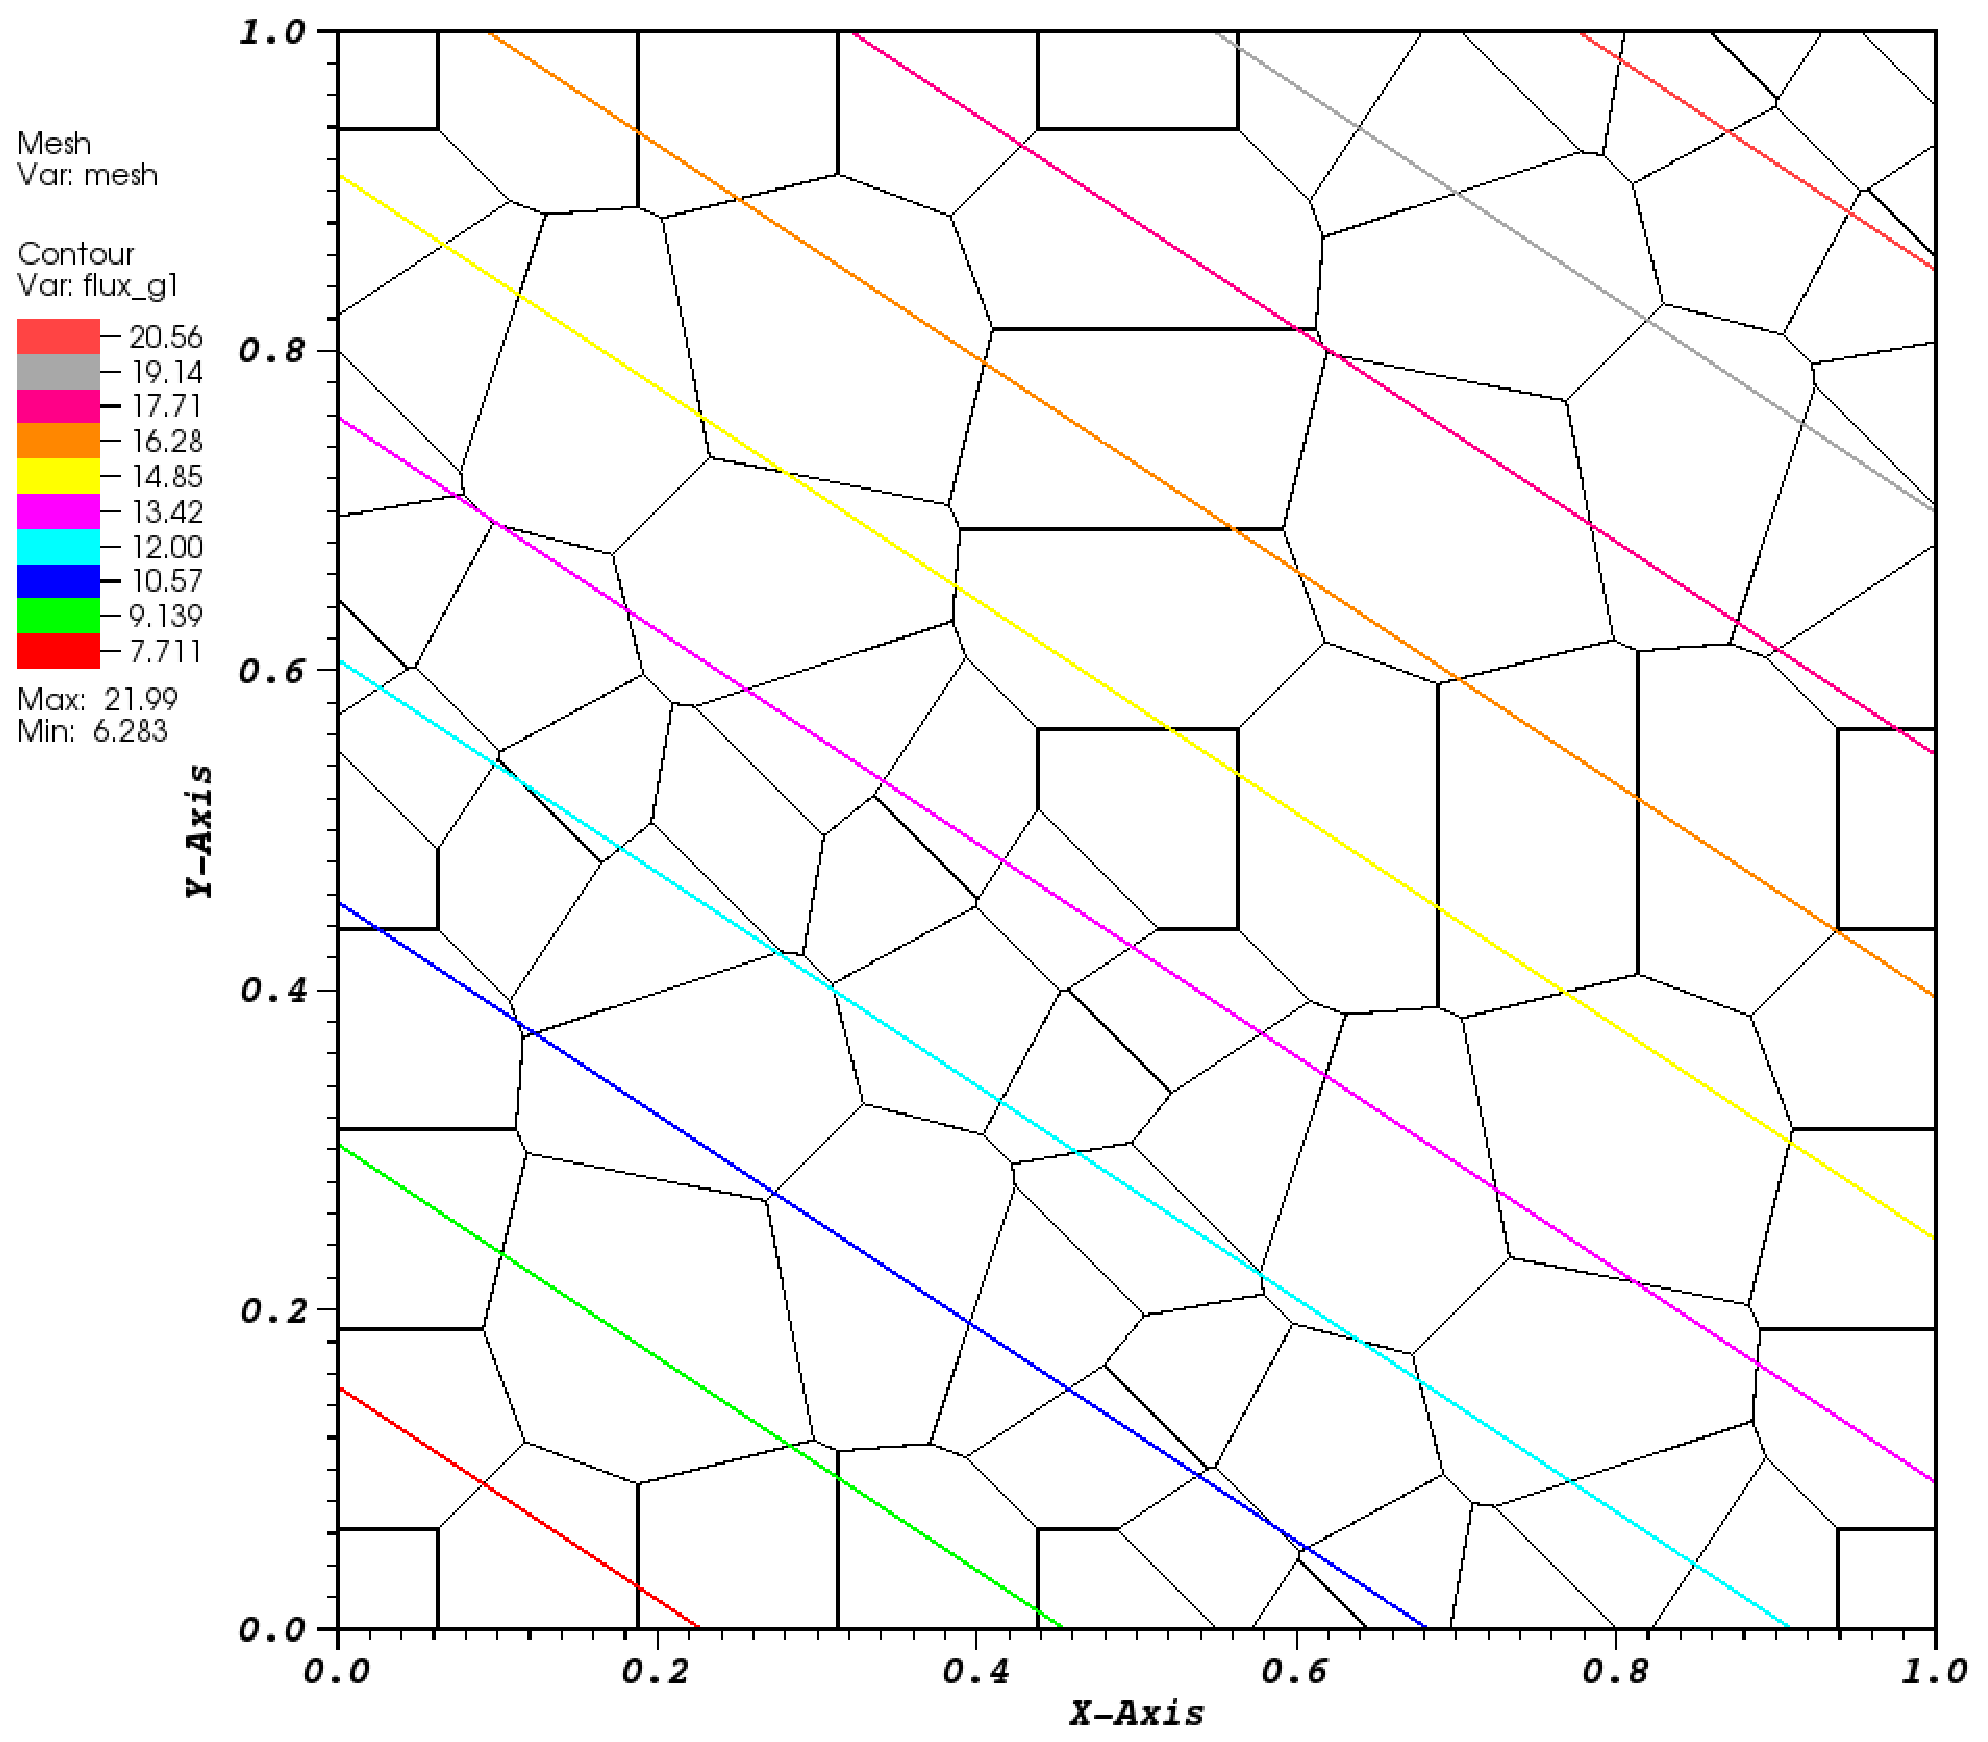
\includegraphics[width=\textwidth]{figures/smooth_poly_PWLD_k1.eps}
		\caption{}
	\end{subfigure}
	\hfill
	\begin{subfigure}[b]{0.42\textwidth}
		\centering
		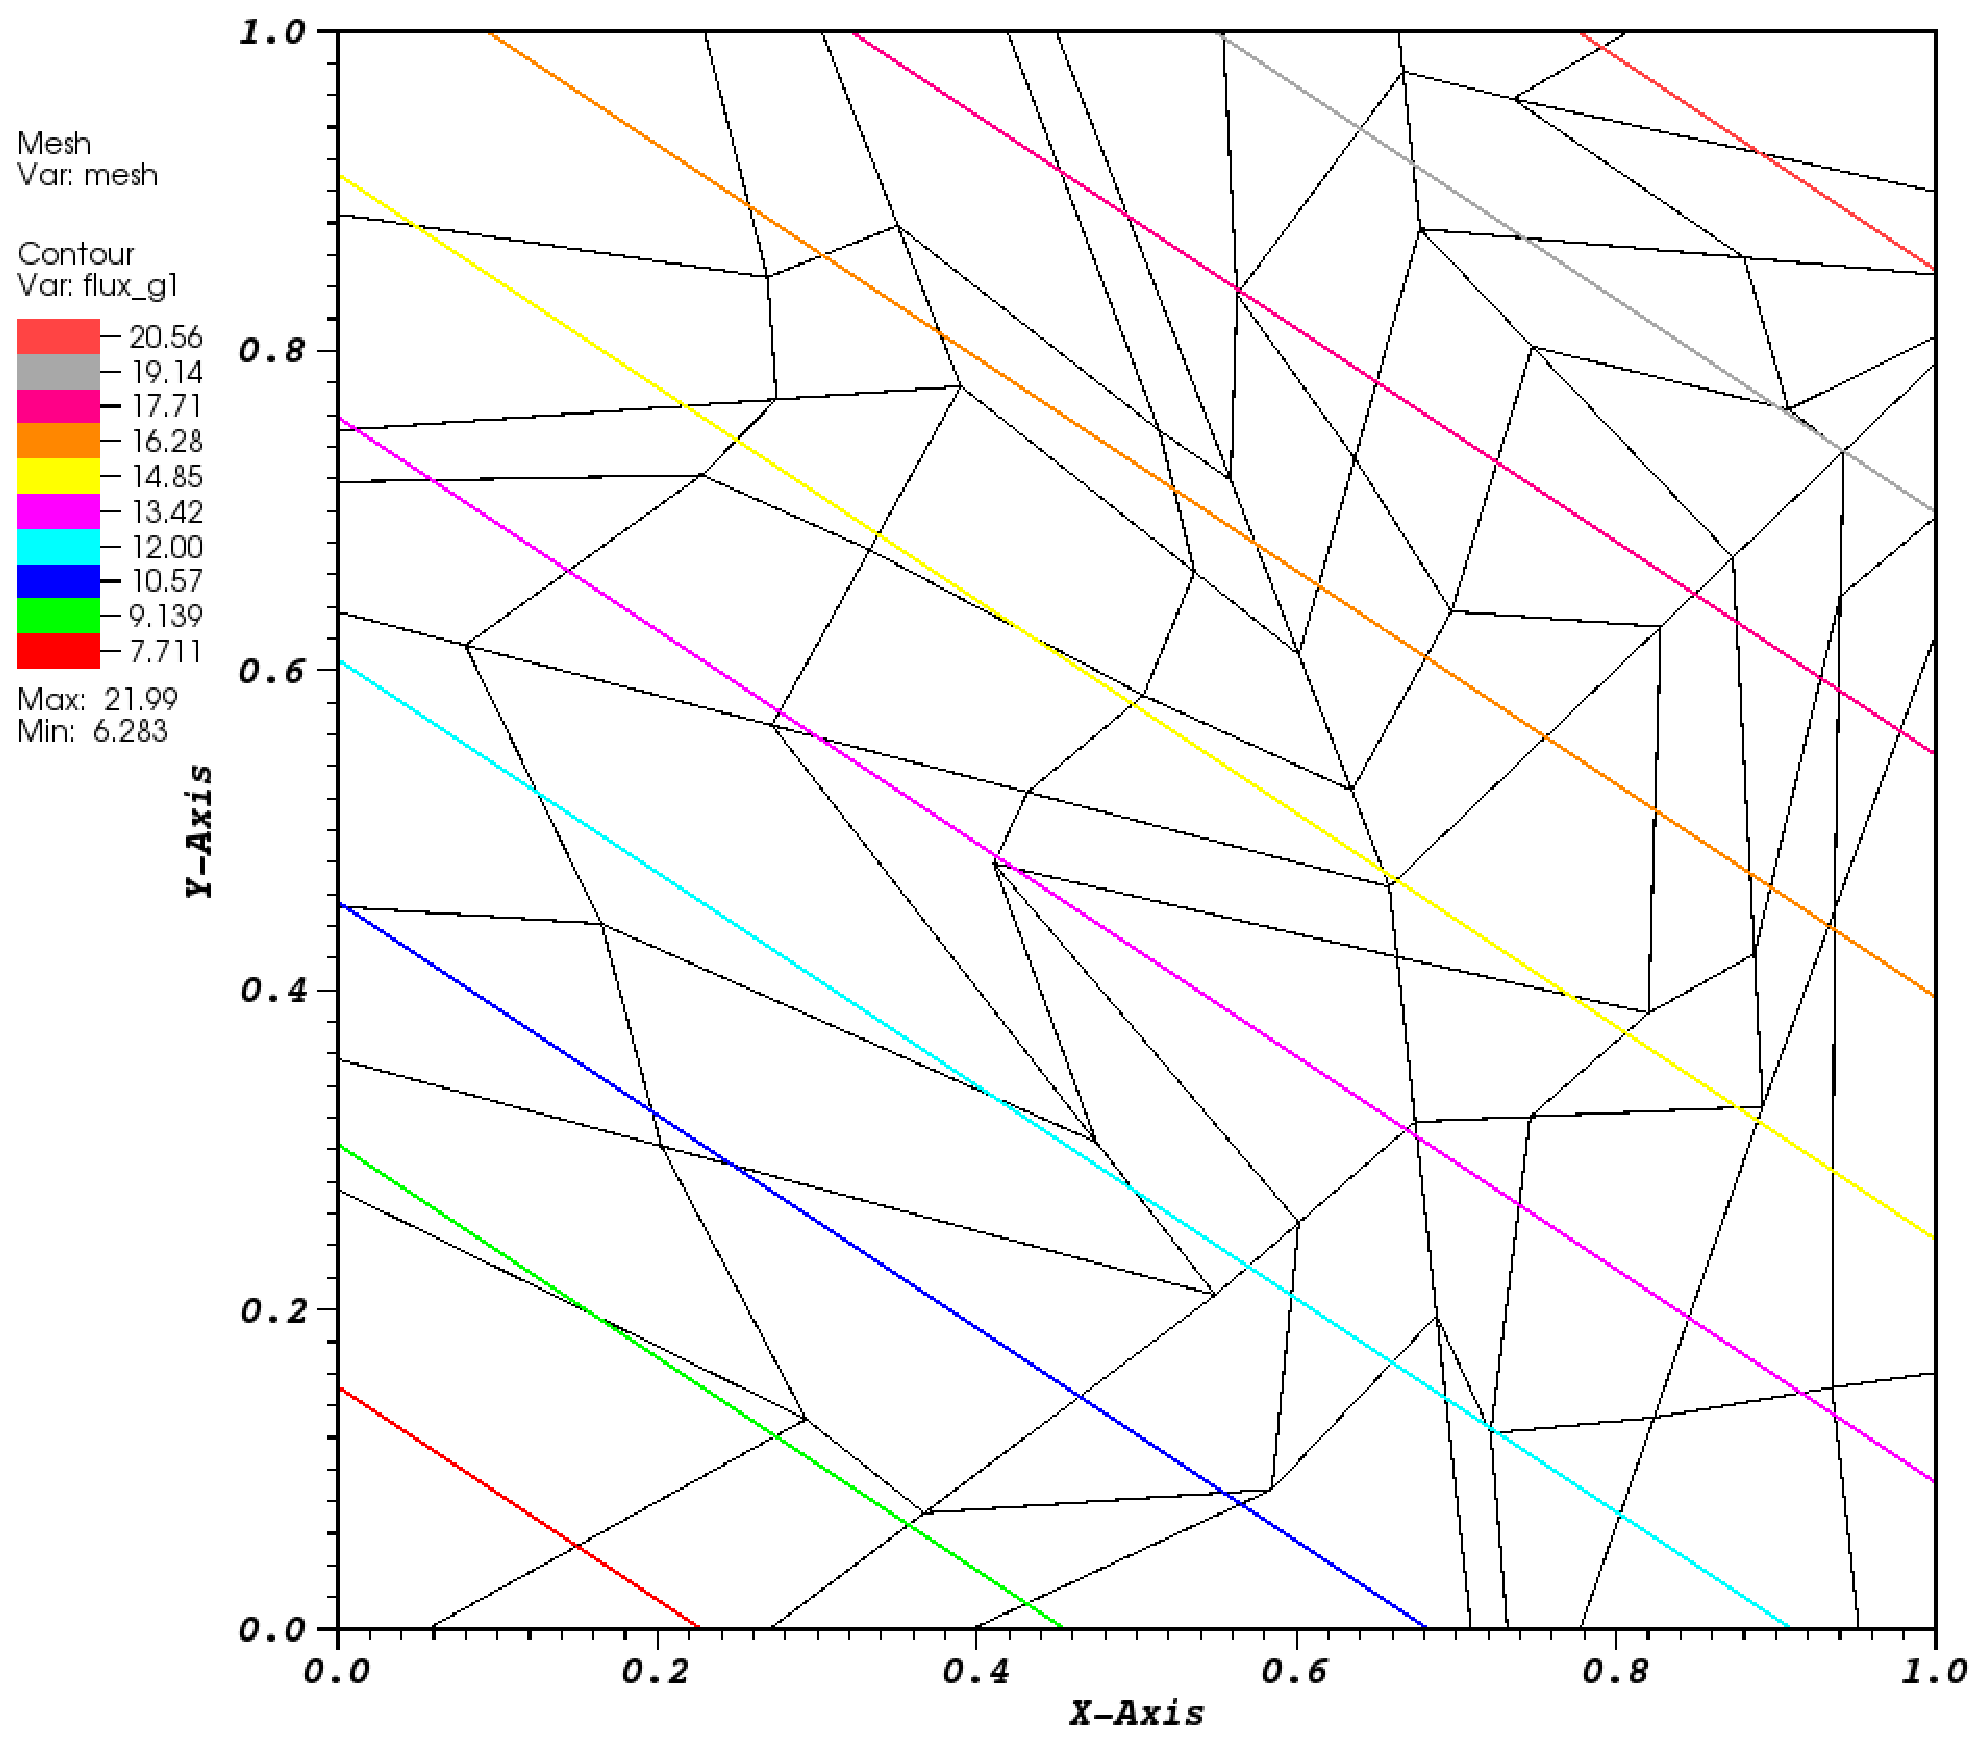
\includegraphics[width=\textwidth]{figures/shes_quad_PWLD_k1.eps}
		\caption{}
	\end{subfigure}
\caption{Exactly linear transport solutions using the PWL coordinates on (a) a sinusoidal polygonal mesh and (b) a highly-distorted quadrilateral shestakov mesh.}
\label{fig::lin_sol}
\end{figure}
\vspace{2mm}

We next want to analyze the convergence rate properties of transport solutions using the different basis functions on polygonal meshes. We will do this by use of the method of manufactured solutions (MMS) \cite{salari2000code}. We will use two different functional forms. First, we analyze a smoothly varying, $C^{\infty}$ analytical solution of the form,

\begin{equation}
\label{eq::sin_eq}
\begin{aligned}
	\Psi(x,y) = &\sin (\nu \frac{\pi x}{L_x}) \sin (\nu \frac{\pi y}{L_y}), \\
	\Phi(x,y) = 2 \pi &\sin (\nu \frac{\pi x}{L_x}) \sin (\nu \frac{\pi y}{L_y}),
\end{aligned}
\end{equation}

\noindent where in this case, the frequency parameter, $\nu$, is set to 3. We test the convergence rates of this transport solution using more regular meshes: orthogonal quadrilaterals, ordered triangles, and regular polygons. Figure \ref{fig::mms_err} presents the convergence rates 

We also wish to test a solution that contains an extreme local maximum. We analyze an analytical solution of the form,

\begin{equation}
\label{eq::gauss_eq}
\begin{aligned}
	\Psi (x,y) = & C_M x (L_x - x) y (L_y - y) \exp(-\frac{(x-x_0)^2 + (y-y_0)^2}{\gamma}) \\ 
	\Phi (x,y) = 2 \pi & C_M x (L_x - x) y (L_y - y) \exp(-\frac{(x-x_0)^2 + (y-y_0)^2}{\gamma})
\end{aligned} \, ,
\end{equation}

\noindent where the equation constant and the deviation parameter are

\begin{equation}
\label{eq::gaussconsts}
C_M = \frac{100}{L_x^2 L_y^2} \qquad \text{and} \qquad \gamma = \frac{L_x L_y}{100} ,
\end{equation}

\noindent respectively. However, for this transport solution, we will utilize adaptive mesh refinement strategies 

\begin{figure}[hbt]
\centering
	\begin{subfigure}[b]{0.485\textwidth}
		\centering
		\includegraphics[width=\textwidth]{figures/cart_err_rev1.eps}
		\caption{}
	\end{subfigure}
	\hfill
	\begin{subfigure}[b]{0.49\textwidth}
		\centering
		\includegraphics[width=\textwidth]{figures/poly_err_rev1.eps}
		\caption{}
	\end{subfigure}
\caption{$L_2$ error norm for the sinusoidal MMS problem using the various 2D polygonal basis functions on (a) orthogonal quadrilateral meshes and (b) random polygonal meshes.}
\label{fig::mms_err}
\end{figure}

\begin{figure}[!hbt]
\centering
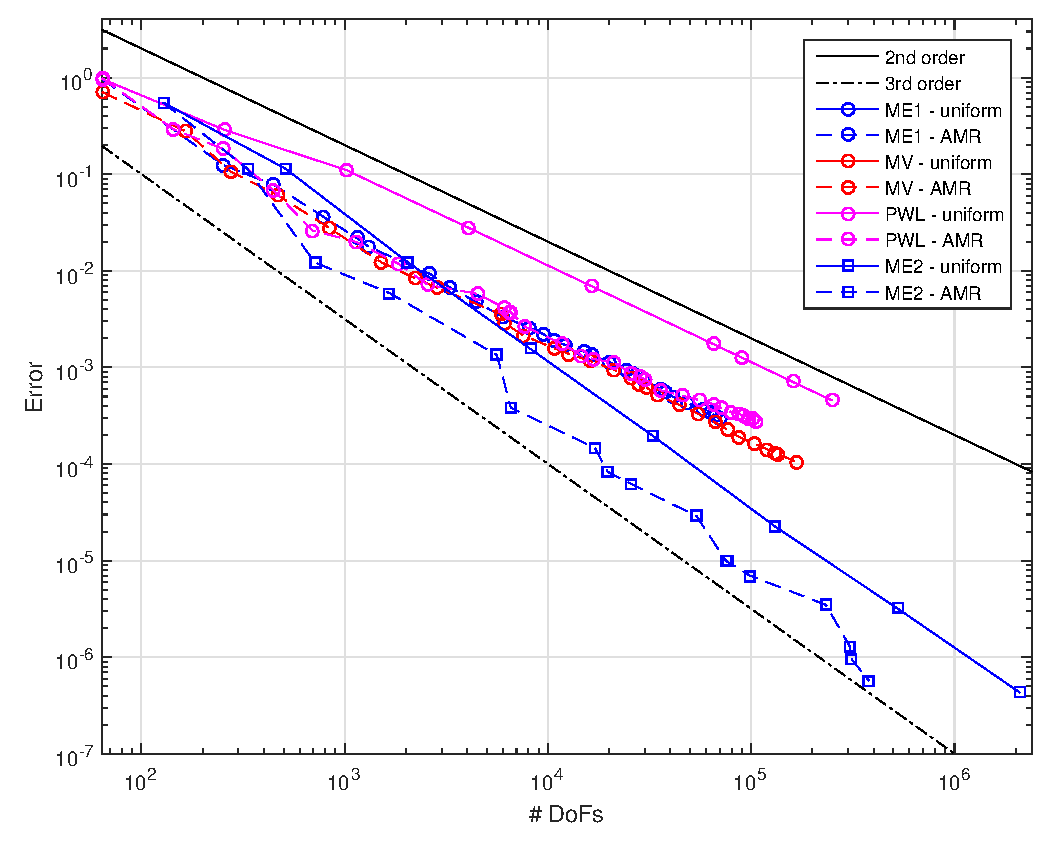
\includegraphics[width=0.6\textwidth]{figures/Transport_Gauss_2D_AMR_Error_Plot.eps}
\caption{$L_2$ error norm for the gaussian MMS problem using the various 2D polygonal basis functions }
\label{fig::Gauss_AMR_err}
\end{figure}

\begin{figure}[hbt]
\centering
	\begin{subfigure}[b]{0.40\textwidth}
		\centering
		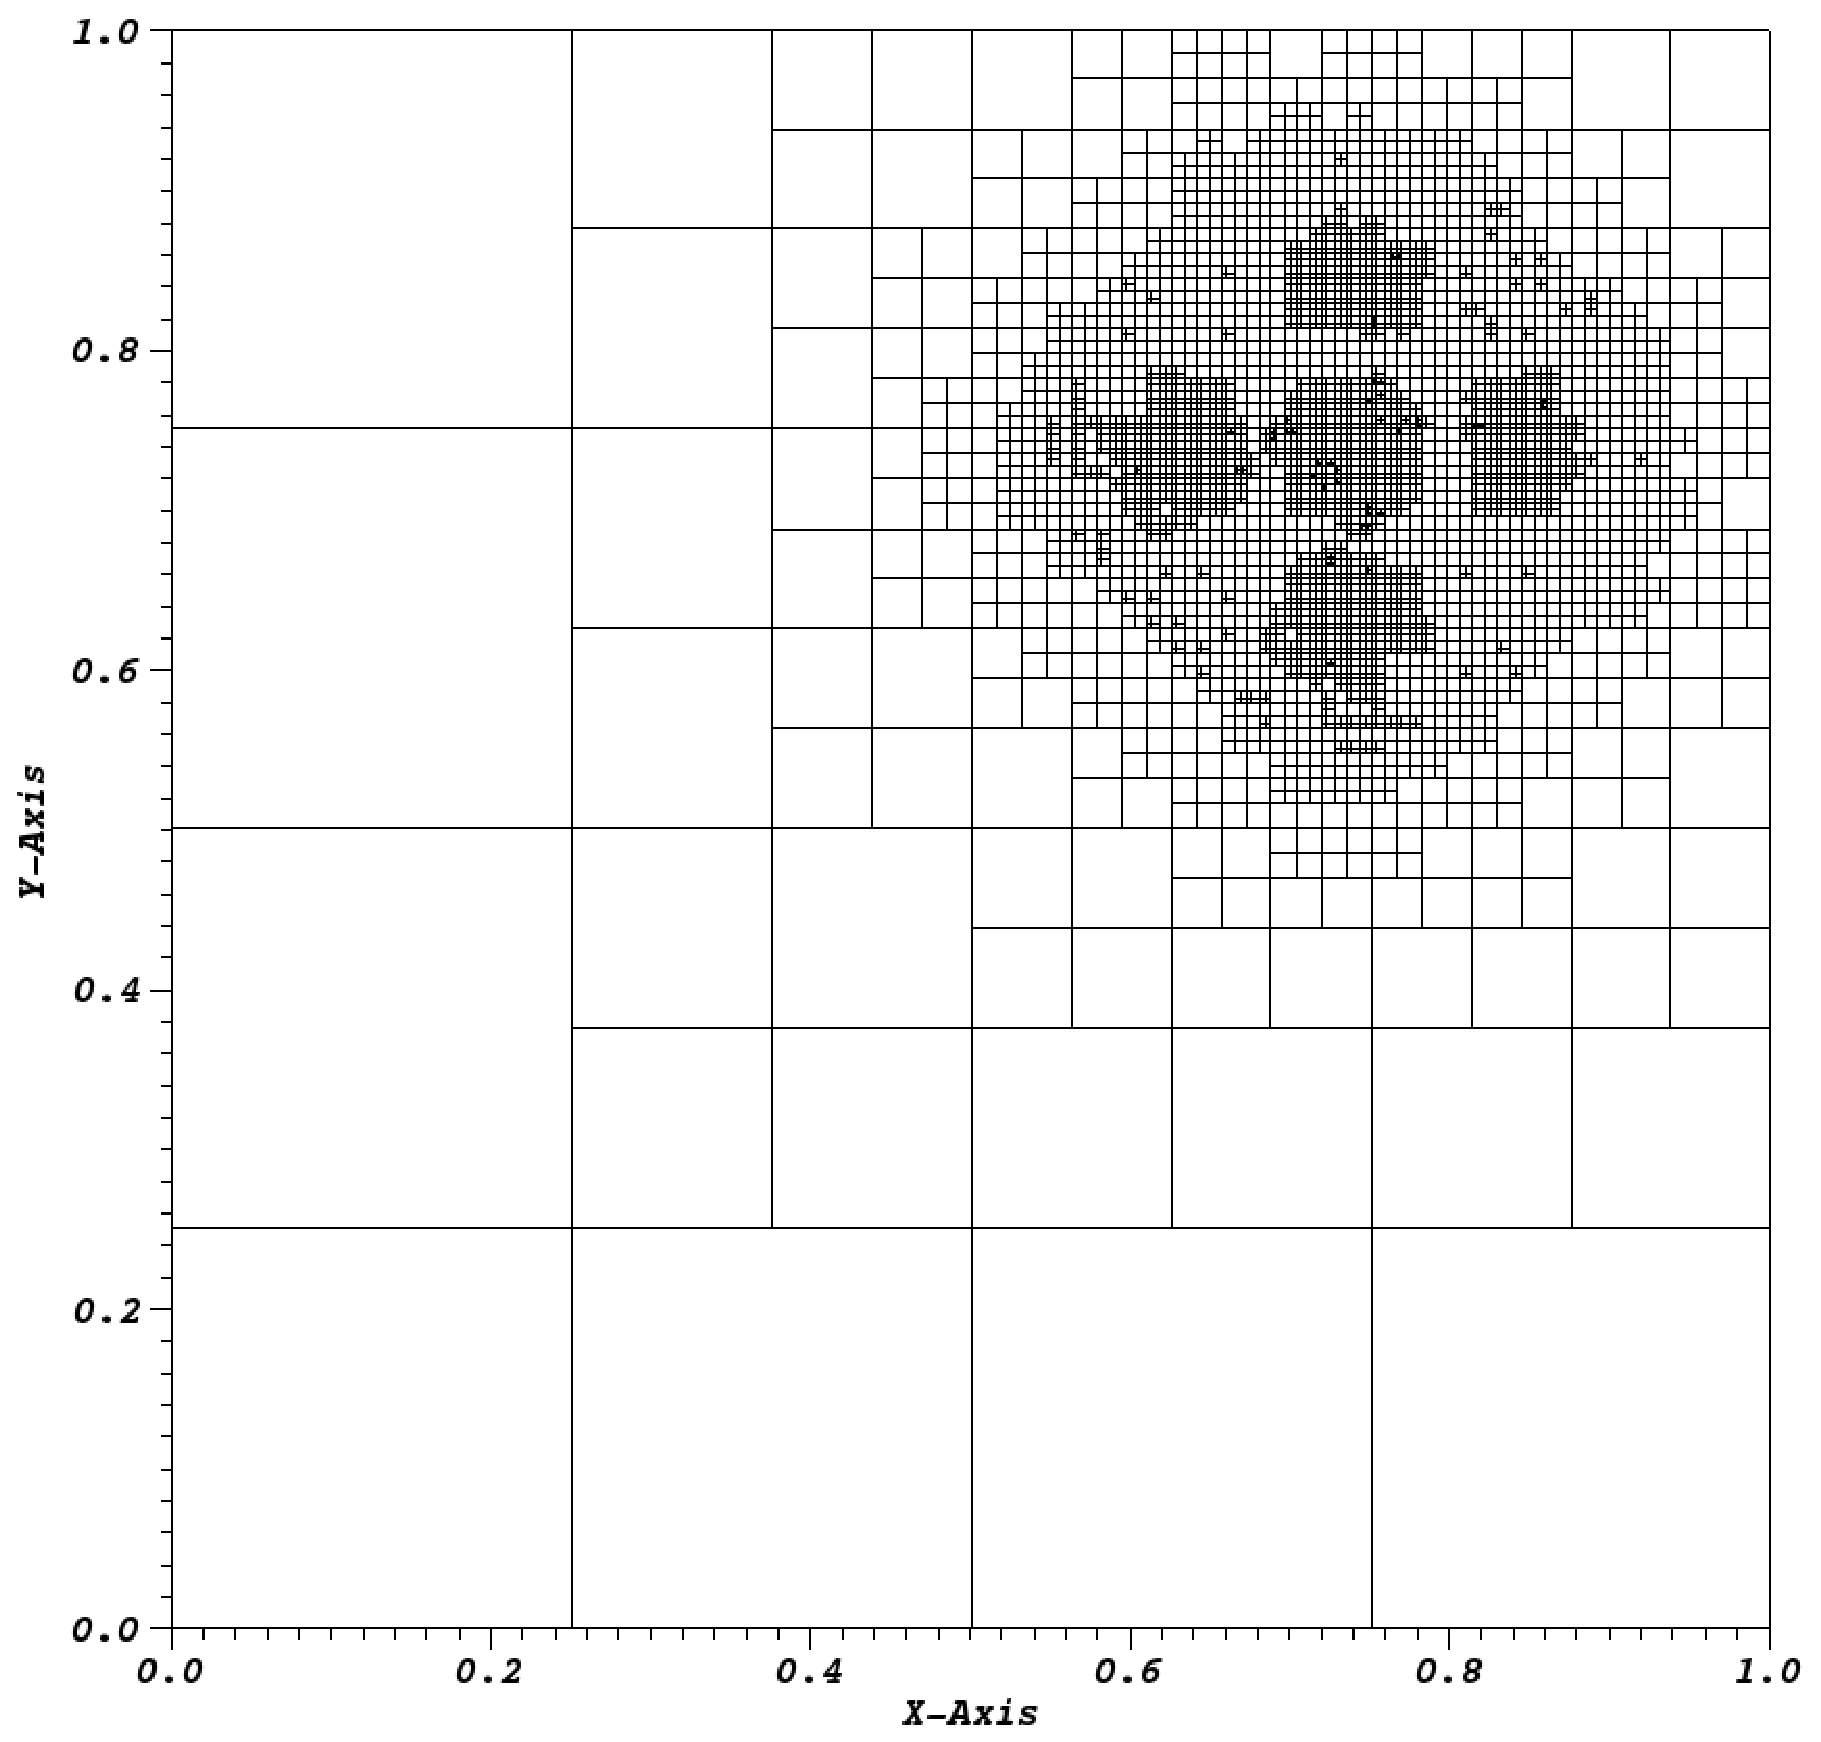
\includegraphics[width=\textwidth]{figures/ME1_cart_mesh.eps}
	\end{subfigure}
	\hspace{1cm}
	\begin{subfigure}[b]{0.40\textwidth}
		\centering
		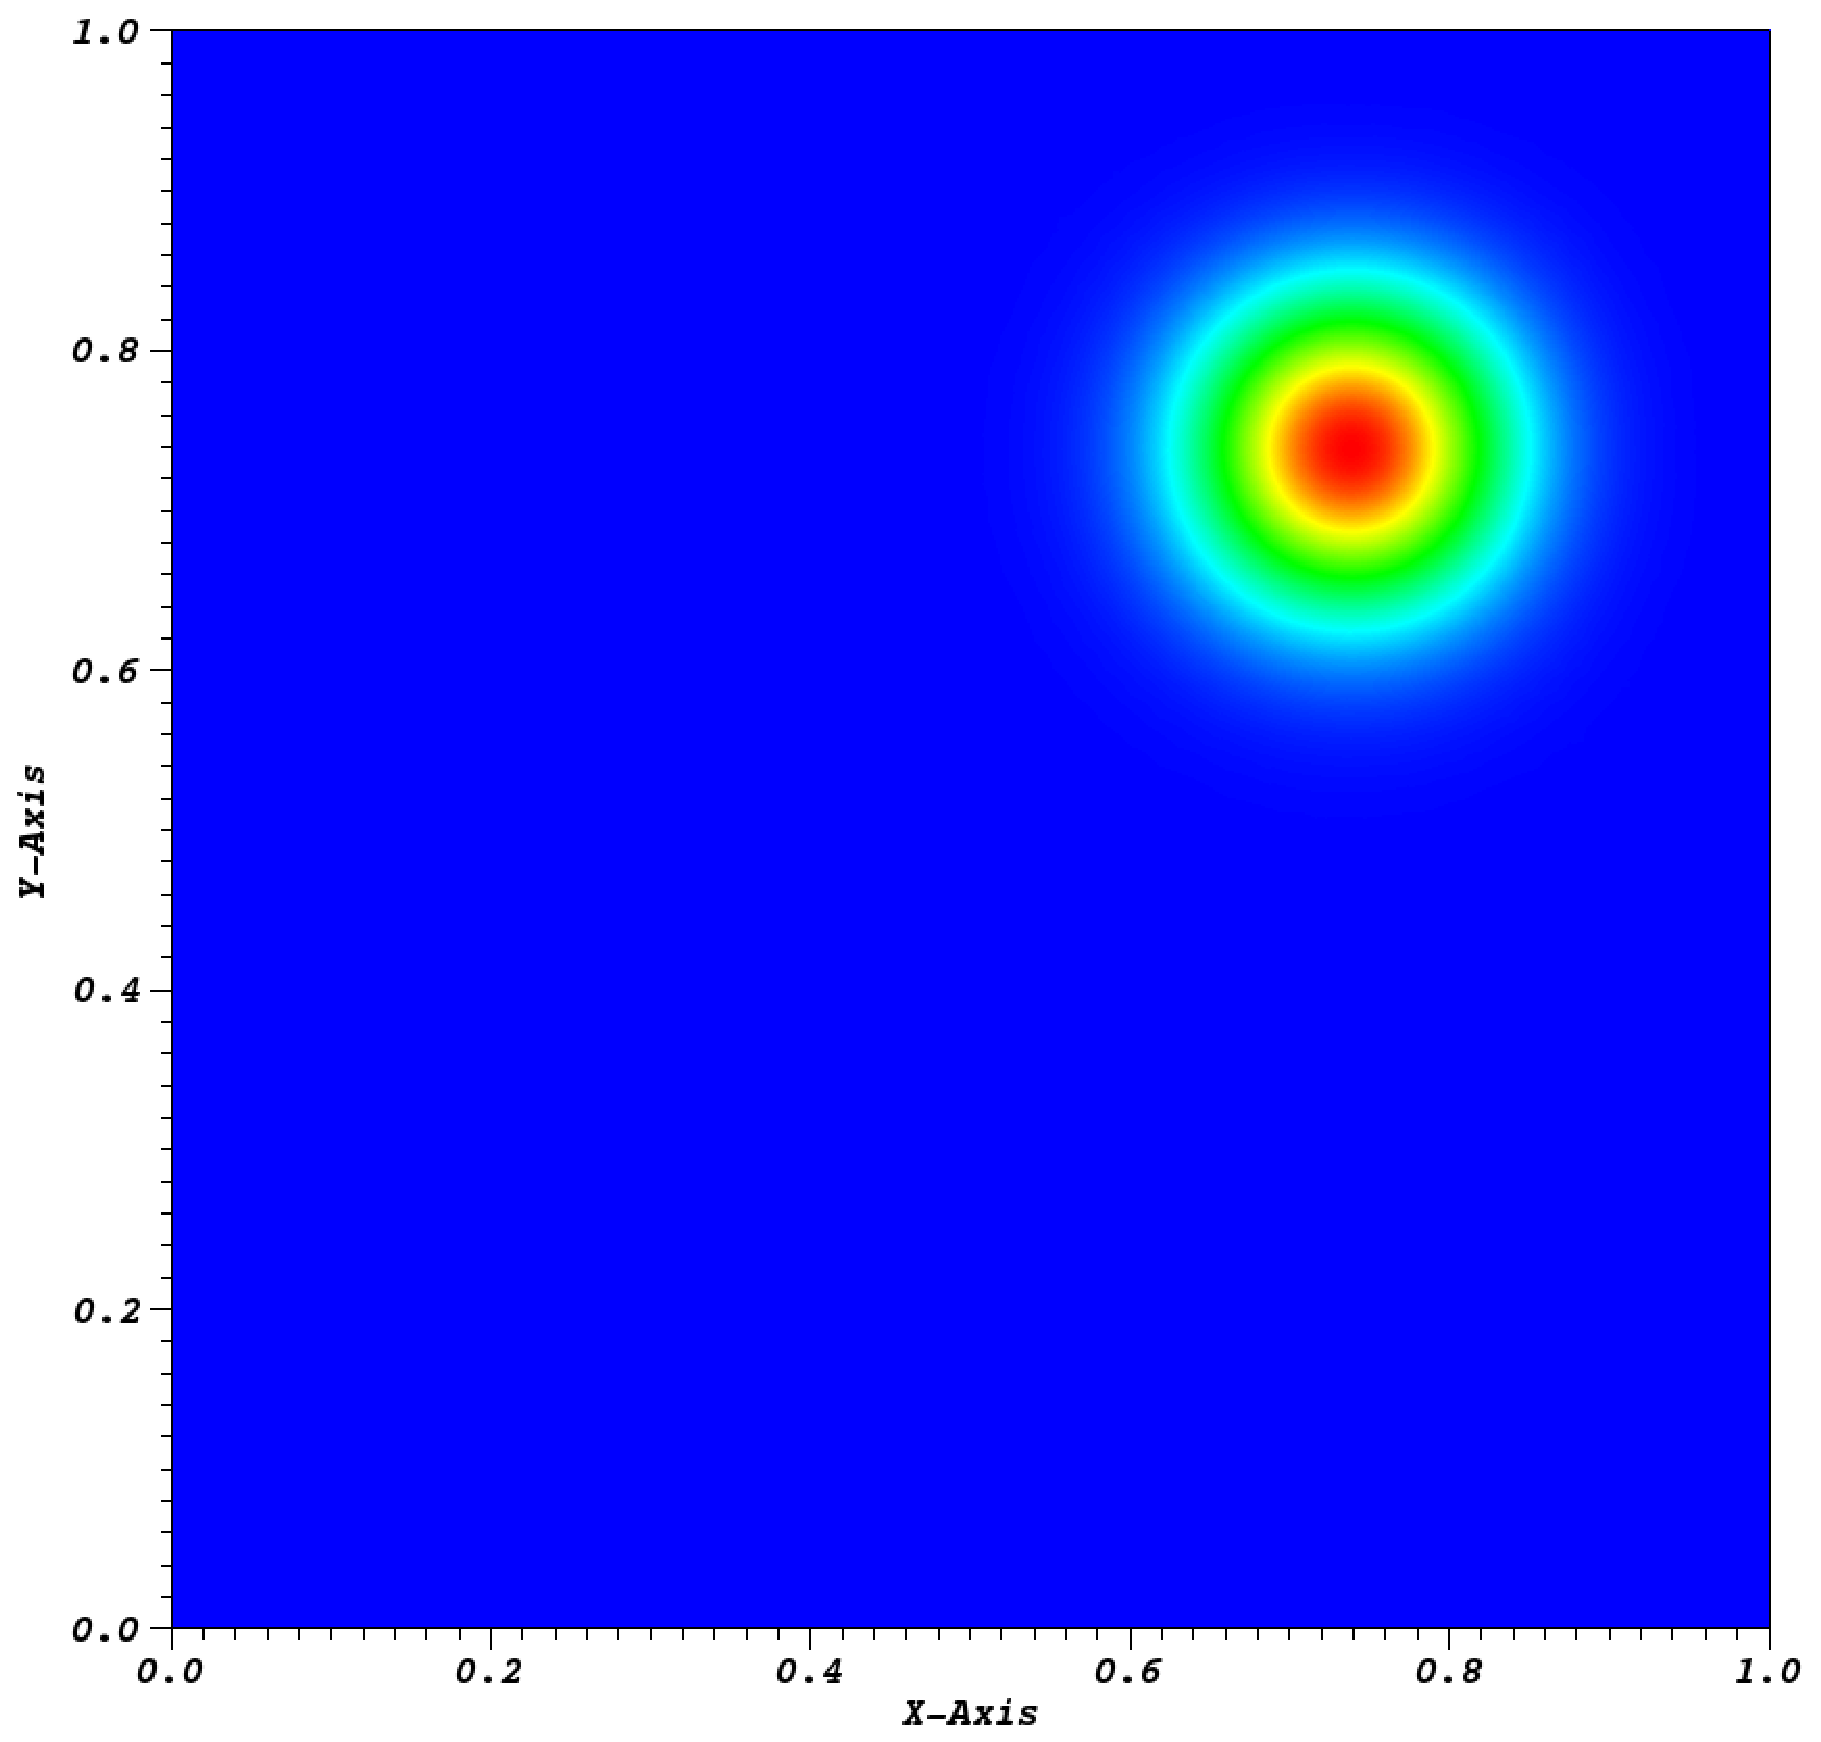
\includegraphics[width=\textwidth]{figures/ME1_cart_sol.eps}
	\end{subfigure}
	\par\bigskip
	\begin{subfigure}[b]{0.40\textwidth}
		\centering
		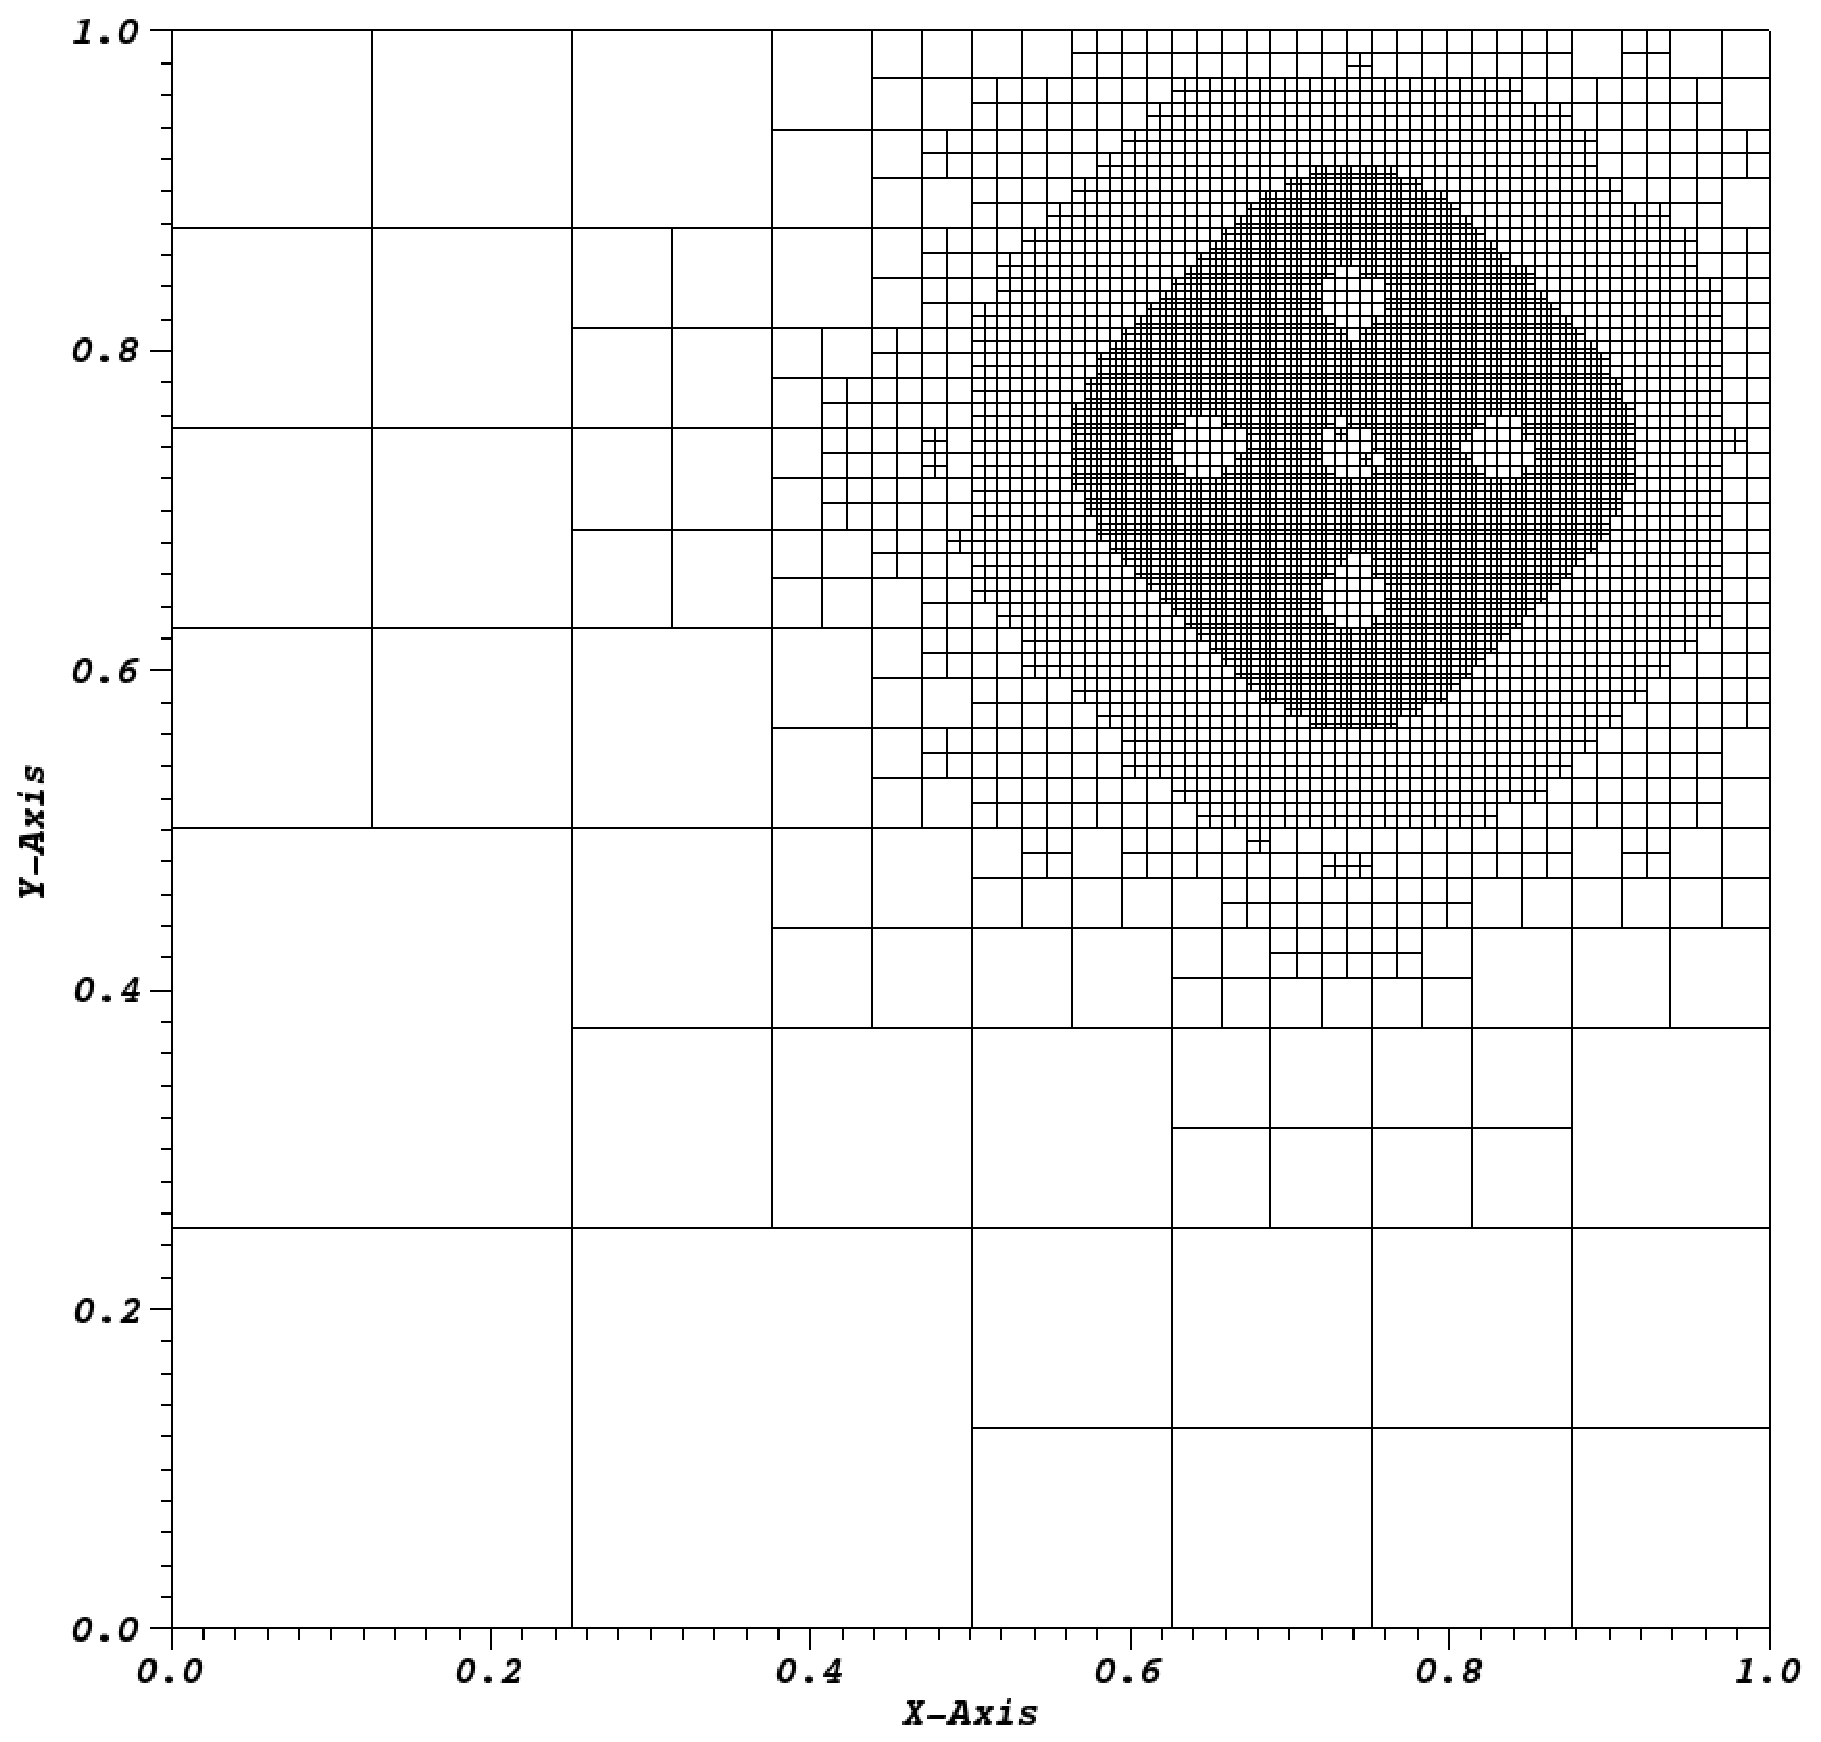
\includegraphics[width=\textwidth]{figures/ME2_cart_mesh.eps}
	\end{subfigure}
	\hspace{1cm}
	\begin{subfigure}[b]{0.40\textwidth}
		\centering
		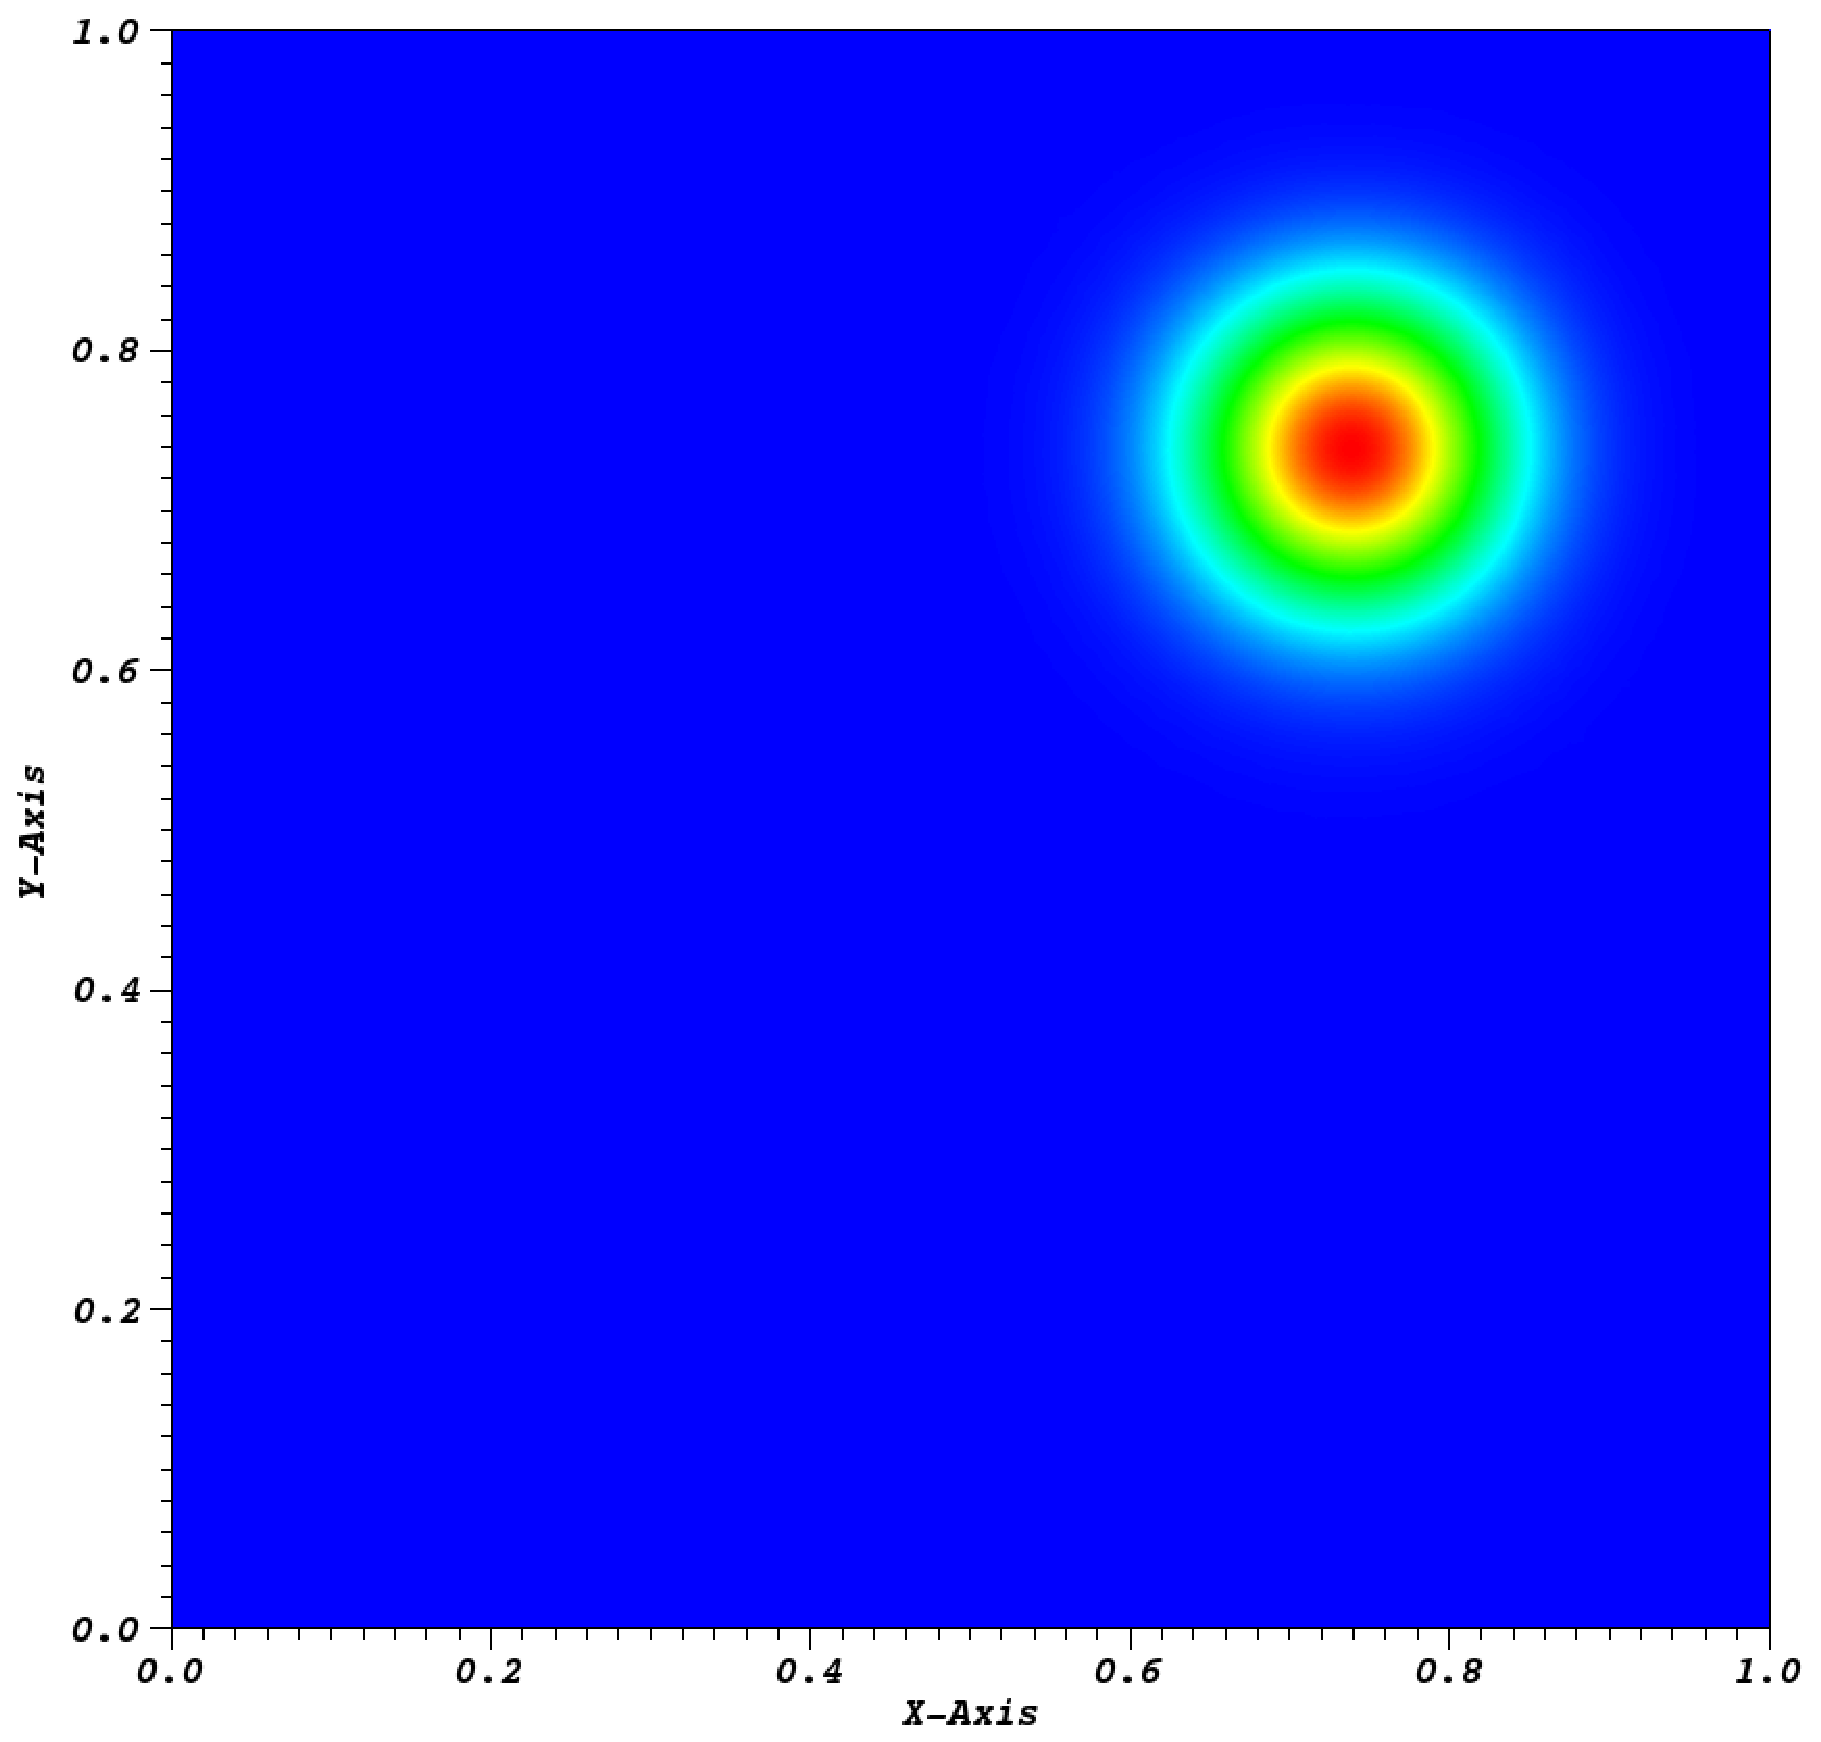
\includegraphics[width=\textwidth]{figures/ME2_cart_sol.eps}
	\end{subfigure}
\caption{AMR meshes and solution plots using the linear maximum entropy coordinates at cycle 15 (top) and the quadratic serendipity maximum entropy coordinates at cycle 08 (bottom).}
\label{fig::AMR_plots}
\end{figure}

%%%%%%%%%%%%%%%%%%%%%%%%%%%%%%%%%%%%%%%%%%%%%%%%%%%%%%%%%%%%%%%%%%%%%%
\subsection{Diffusion Synthetic Acceleration for Massively-Parallel Problems}
\label{sec::CW_DSA}

As it was previously stated, efficient methods for inverting the streaming operator do not guarantee efficiency in solving the transport problem for optically thick configurations. 

\begin{equation}
\label{eq::CW_trans_eq}
\begin{aligned}
{\bf A} \Psi &= {\bf B} \Phi +  {\bf C} \Phi + {\bf Q} \\
\Phi &= {\bf D} \Psi
\end{aligned}
\end{equation}

\noindent where ${\bf A}$, ${\bf B}$, ${\bf C}$, and ${\bf Q}$ are different operators of the transport problem. We then define an iterative procedure of the form,

\begin{equation}
\label{eq::CW_trans_eq_it}
{\bf A} \Psi^{(k+1/2)} = {\bf B} \Phi^{(k+1/2)} + {\bf C} \Phi^{(k)} + {\bf Q},
\end{equation}

\noindent where ${\bf B}$ operates on the current solution iterate and ${\bf C}$ operates on the previous solution iterate. We then subtract Eq. (\ref{eq::CW_trans_eq_it}) from Eq. (\ref{eq::CW_trans_eq}) to yield the following formulation of the solution error at iterate $(k+1/2)$,

\begin{equation}
\label{eq::CW_trans_eq_it_diff}
{\bf A} \delta \Psi^{(k+1/2)} = {\bf B}' \delta \Phi^{(k+1/2)} + {\bf R}^{(k+1/2)}, 
\end{equation}

\noindent where
\begin{equation}
\label{eq::CW_delta_fluxes}
\begin{aligned}
\delta \Psi^{(k+1/2)} &\equiv  \Psi - \Psi^{(k+1/2)} \\
\delta \Phi^{(k+1/2)} &\equiv {\bf D} \delta \Psi^{(k+1/2)}
\end{aligned} \, ,
\end{equation}

\noindent are the errors in the angular fluxes and flux moments, ${\bf R}^{(k+1/2)}$ is some residual in the error, and the operators ${\bf B}$ and ${\bf B'}$ are not necessarily the same. If we could exactly solve for the error in Eqs. (\ref{eq::CW_trans_eq_it_diff} - \ref{eq::CW_delta_fluxes}), then the exact solution could be calculated by: $\Phi =  \Phi^{(k+1/2)} + \delta \Phi^{(k+1/2)}$. Unfortunately, Eq. (\ref{eq::CW_trans_eq_it_diff}) is just as difficult to solve as Eq. (\ref{eq::CW_trans_eq}). Therefore, we estimate Eq. (\ref{eq::CW_trans_eq_it_diff}) with a low-order operator that is easy to solve.


%%%%%%%%%%%%%%%%%%%
\subsubsection{Modified Interior Penalty Diffusion Form for DSA Preconditioning}
\label{sec::CW_DSA_MIP}

As previously stated in Section \ref{sec::PS}, the diffusion operator has been utilized in different forms for the low-order operators of Eq. (\ref{eq::CW_trans_eq_it_diff}). As mentioned, the MIP DSA form has many beneficial properties and it has been extensively analyzed for 2D transport problems \cite{ref::DSA_wang_ragusa,turcksin2014discontinuous}. In this dissertation work, we will extend the MIP DSA analysis to 3D transport problems. We will also extensively analyze the scalability 

The MIP diffusion form is defined with the following bilinear left-hand-side,

\begin{equation}
\label{eq::mip_lhs}
\begin{aligned}
a(\delta \Phi, b)  = \Big<  D \vec{\nabla} \delta  \Phi , \vec{\nabla} b \Big>_{\mathcal{D}} + \Big<  \sigma \delta  \Phi , b  \Big>_{\mathcal{D}}    \\
+  \Big\{ \kappa_e^{MIP} [\![ \delta  \Phi ]\!] , [\![  b ]\!]\Big\}_{E_h^i} + \Big\{  [\![  \delta \Phi ]\!] , \{\!\{  D \partial_n b \}\!\}\Big\}_{E_h^i}  + \Big\{ \{\!\{  D \partial_n \delta \Phi \}\!\} , [\![ b ]\!]\Big\}_{E_h^i} \\
+ \Big\{ \kappa_e^{MIP}  \delta \Phi ,   b \Big\}_{\partial \mathcal{D}^{vac}} - \frac{1}{2} \Big\{  \delta \Phi  ,  D \partial_n b \Big\}_{\partial \mathcal{D}^{vac}} - \frac{1}{2} \Big\{   D \partial_n \delta  \Phi , b \Big\}_{\partial \mathcal{D}^{vac}}  
\end{aligned} ,
\end{equation}

\noindent and with the following linear right-hand-side,

\begin{equation}
\label{eq::mip_rhs}
\ell(b) = \Big<  R, b  \Big>_{\mathcal{D}} + \Big\{ \delta  J^{inc}, b \Big\}_{\partial \mathcal{D}^{ref}} .
\end{equation}

\noindent The MIP penalty coefficient, $\kappa_e^{MIP}$, has the form:

\begin{equation}
\label{eq::ip_penalty}
\kappa_e^{MIP} = \max(\frac{1}{4}, \kappa_e^{IP}) , \qquad
\kappa_e^{IP}  \equiv 
		\begin{cases}
		\frac{C_B}{2} \left(  \frac{D^+}{h^+} + \frac{D^-}{h^-}  \right) & , e \in E_h^i \\
		C_B \frac{D^-}{h^-}  & , e \in \partial \mathcal{D}
		\end{cases} \, ,
\end{equation}

\noindent where $C_B=cp(p+1)$, $c$ is a user defined constant ($c \geq 1$), $p$ is the polynomial order of the basis function, $D^{\pm}$ are the diffusion coefficients on either side of face $e$ and $h^{\pm}$ are the orthogonal projections on either side of face $e$. We determine the positive and negative cells by the following trace:

\begin{equation}
\label{eq::mip_trace}
u^{\pm} = \lim_{s \rightarrow 0^{\pm}} u (\vec{r} + s \vec{n}) .
\end{equation}

\noindent For interior faces, we can specify an arbitrary direction for the face normal, but boundary faces require the face normals to orient outwards from the domain.

To date, we have carried out extensive analysis for both 2D and 3D MIP DSA preconditioning.

\begin{figure}[hbt]
\centering
	\begin{subfigure}[b]{0.48\textwidth}
		\centering
		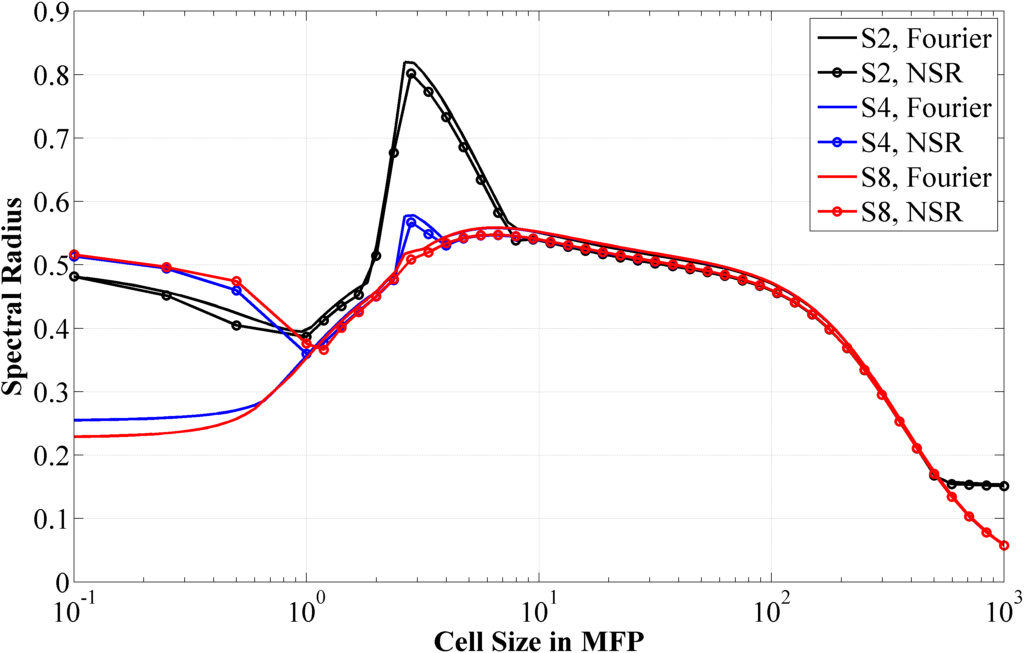
\includegraphics[width=\textwidth]{figures/SI_MIP_hex_C=1_LS2,4,8_F&NSR_PDT.png}
	\end{subfigure}
	\hfill
	\begin{subfigure}[b]{0.48\textwidth}
		\centering
		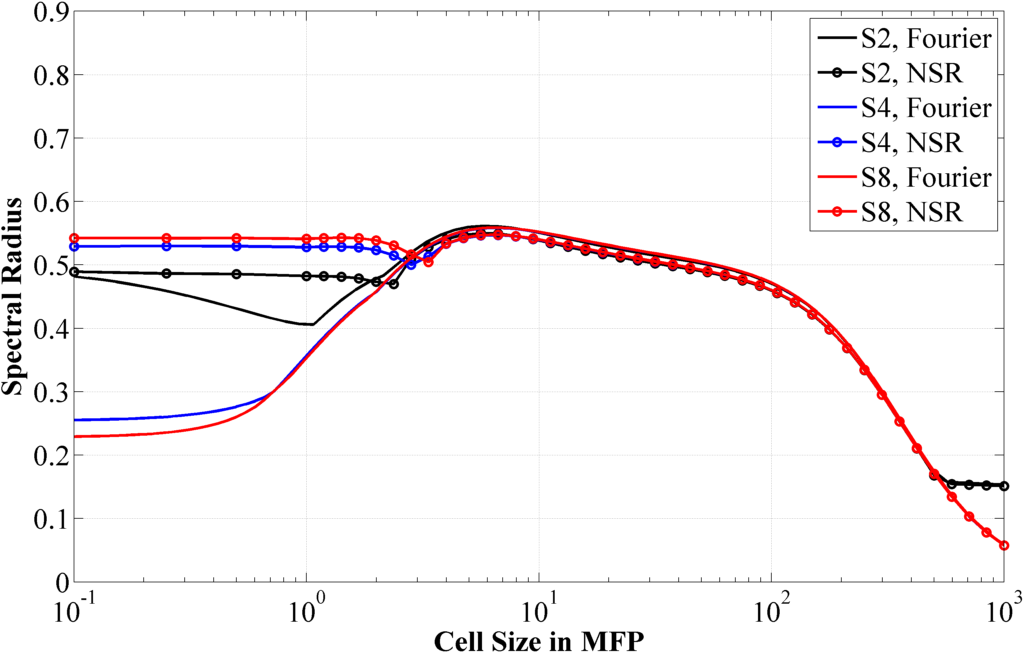
\includegraphics[width=\textwidth]{figures/SI_MIP_hex_C=4_LS2,4,8_F&NSR_PDT.png}
	\end{subfigure}
	\vfill
	\begin{subfigure}[b]{0.48\textwidth}
		\centering
		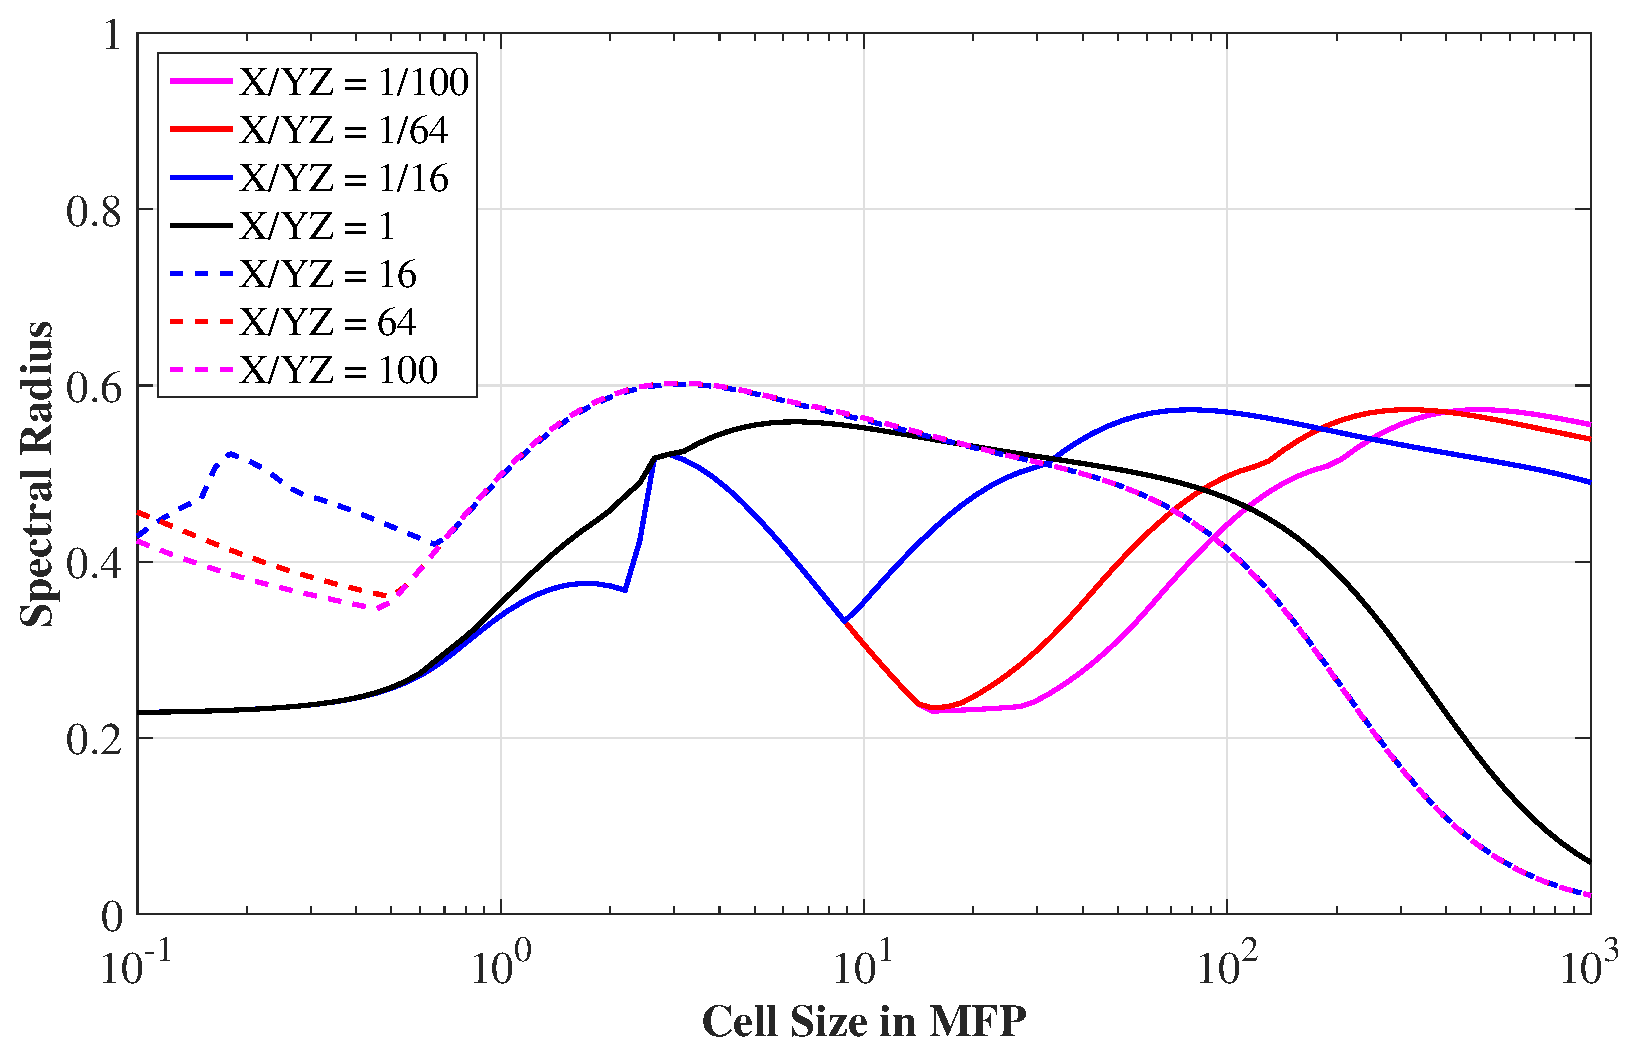
\includegraphics[width=\textwidth]{figures/SI_MIP_hex_LS8_C=1_AR.eps}
	\end{subfigure}
	\hfill
	\begin{subfigure}[b]{0.48\textwidth}
		\centering
		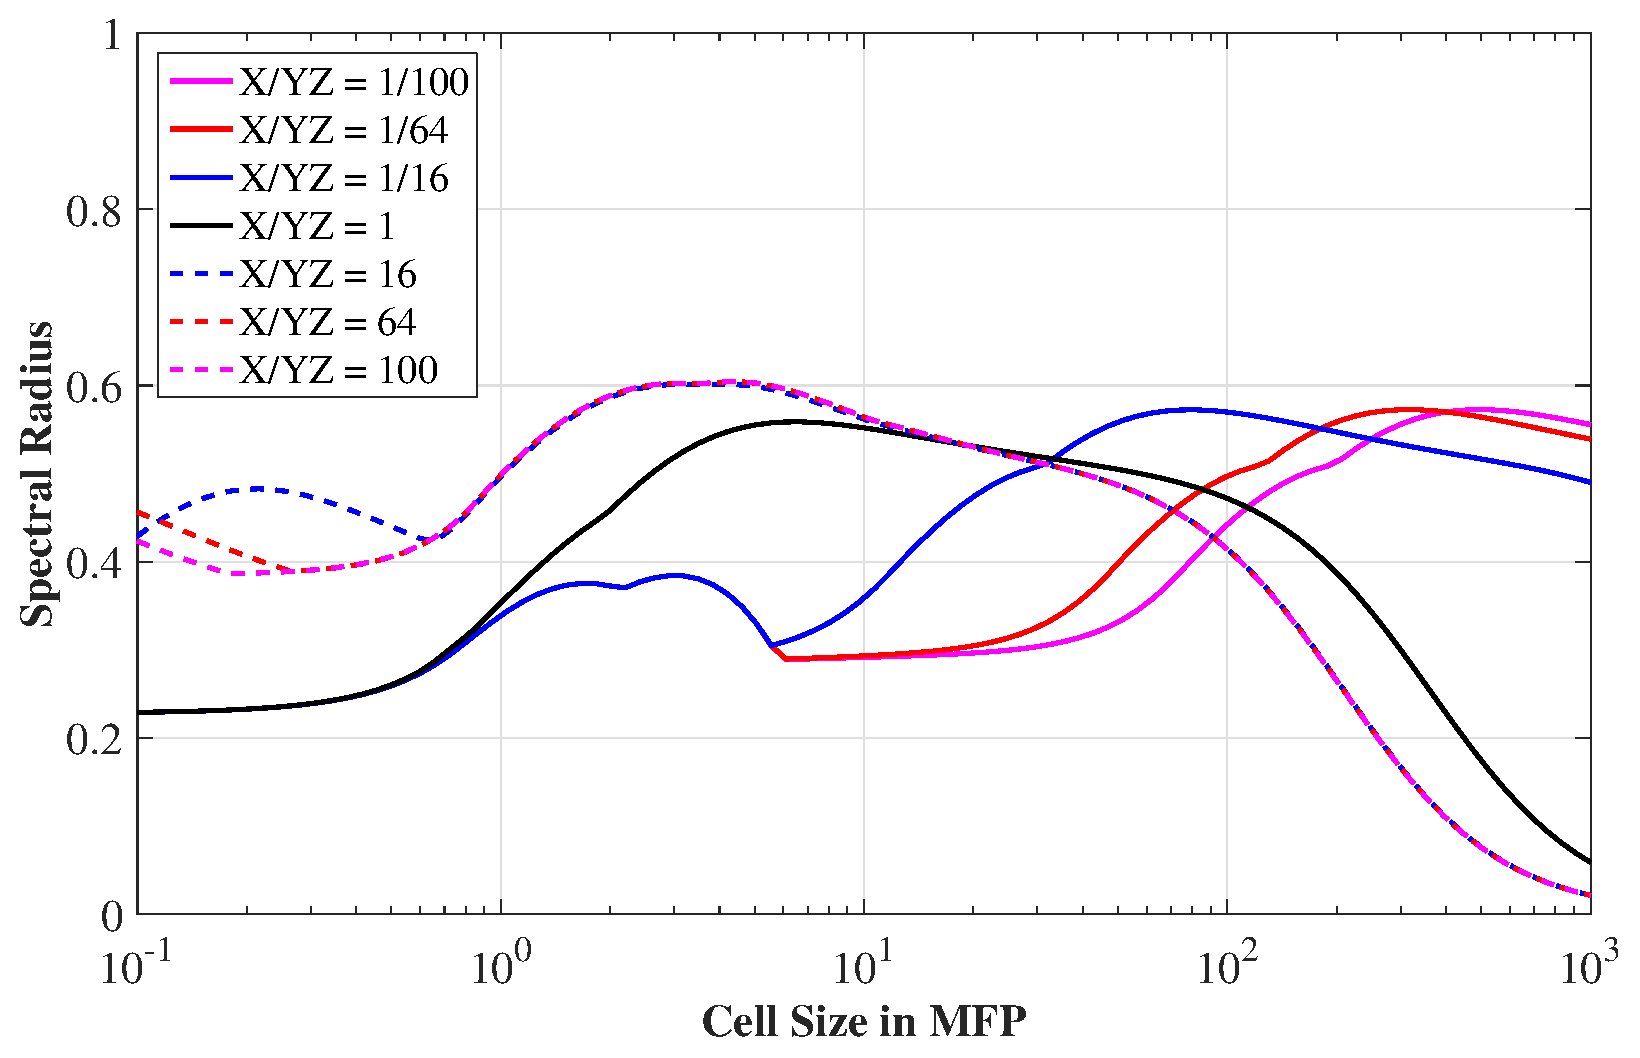
\includegraphics[width=\textwidth]{figures/SI_MIP_hex_LS8_C=4_AR.eps}
	\end{subfigure}
\caption{Fourier and numerical spectral radii results on the unit cube with PWL basis functions and varying $S_N$ order (top). Fourier spectral radii results on parallelipipeds with varying aspect ratios with PWL basis functions and $S_8$ order (bottom). MIP penalty constant: $c=1$ (left) and $c=4$ (right).}
\label{fig::fourier_NSR}
\end{figure}



\begin{figure}[hbt]
\centering
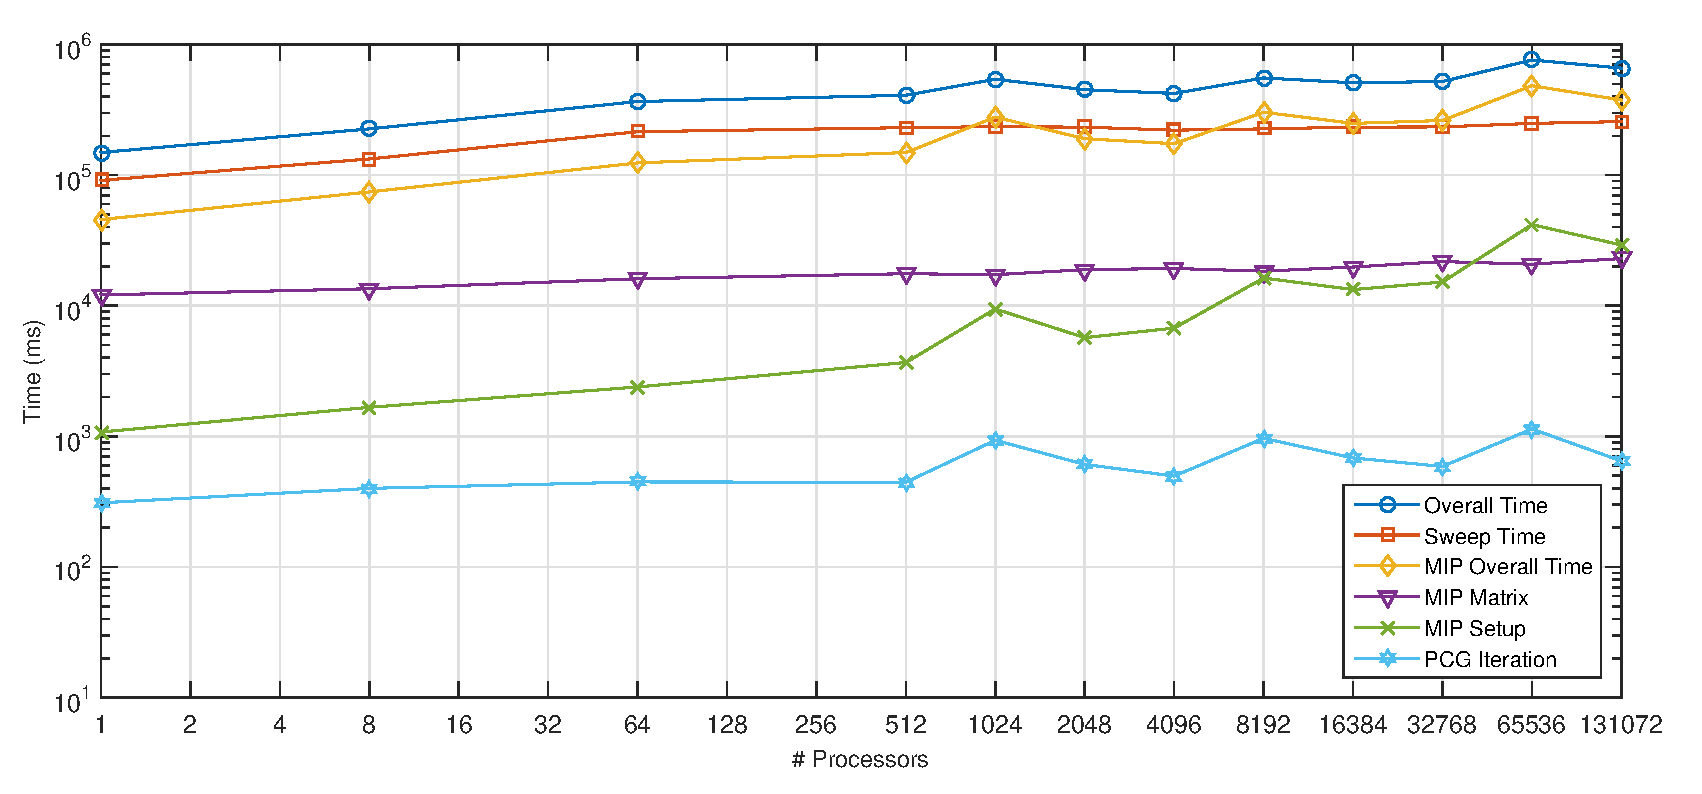
\includegraphics[width=0.85\textwidth]{figures/Vulcan_DSA_Timing.eps}
\caption{Timing data for MIP DSA preconditioning in the PDT code on the VULCAN cluster.}
\label{fig::Vulcan_MIP_Timing}
\end{figure}

%%%%%%%%%%%%%%%%%%%
\subsubsection{Thermal up-scatter Acceleration - Two-Grid DSA Preconditioning}
\label{sec::CW_DSA_TG}

For this dissertation work, we will also analyze the benefits and scalability of DSA preconditioning to real-world problems. This can require the ability to efficiently converge the scattering source for a large multigroup problem. However, if there is appreciable up-scattering from the thermal energy groups, then the system can act optically thick which leads to arbitrarily-slow convergence. In particular, systems that are dominated by the thermal scattering off graphite or heavy-water behave in this manner.

To combat this slow convergence, we will analyze the scalability of the two-grid DSA preconditioning method on high-fidelity real-world problems \cite{adams1993two}. We summarize the two-grid scheme in the following manner. We first write the completely-discretized multigroup $S_N$ equations in simple operator form,

\begin{equation}
\label{eq::MG_full_eq}
{\bf L} \Psi_g =  {\bf M} \sum_{g'=0}^G {\bf S}_{g g'} \Phi_{g'} + {\bf Q}_g,
\end{equation}

\noindent where ${\bf M}$ and ${\bf S}$ are the moment-to-discrete and scattering operators, respectively. We then apply the Gauss-Seidel iteration scheme to Eq. (\ref{eq::MG_full_eq}) to form the following iterative system of equations,

\begin{equation}
\label{eq::GS_it}
{\bf L} \Psi_g^{(k+1/2)} = {\bf M} \sum_{g'=0}^g {\bf S}_{g g'} \Phi_{g'}^{(k+1/2)} + {\bf M} \sum_{g'=g+1}^G {\bf S}_{g g'} \Phi_{g'}^{(k)} + {\bf Q}_g .
\end{equation}

We subtract Eq. (\ref{eq::GS_it}) from Eq. (\ref{eq::MG_full_eq}) to yield the following error equation for the system of Gauss-Seidel equations:

\begin{equation}
\label{eq::GS_error}
{\bf L} \delta \Psi_g^{(k+1/2)} = {\bf M} \sum_{g'=0}^g {\bf S}_{g g'} \delta \Phi_{g'}^{(k+1/2)} + {\bf R}_g^{(k+1/2)}  ,
\end{equation}

\noindent where the residual is of the form:

\begin{equation}
\label{eq::TG_residual}
{\bf R}_g^{(k+1/2)} = {\bf M} \sum_{g'=g+1}^G {\bf S}_{g g'} \left(  \Phi_{g'}^{(k+1/2)} - \Phi_{g'}^{(k)}  \right).
\end{equation}

\begin{figure}
\centering
	\begin{subfigure}[b]{0.49\textwidth}
		\centering
		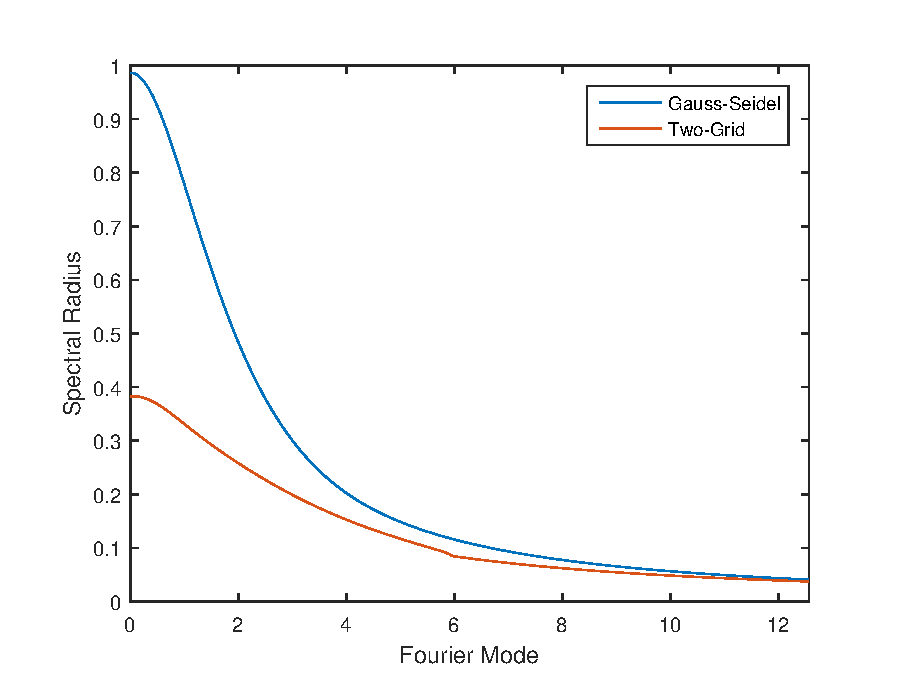
\includegraphics[width=\textwidth]{figures/P0_Fourier_69G.eps}
		\caption{}
	\end{subfigure}
	\hfill
	\begin{subfigure}[b]{0.49\textwidth}
		\centering
		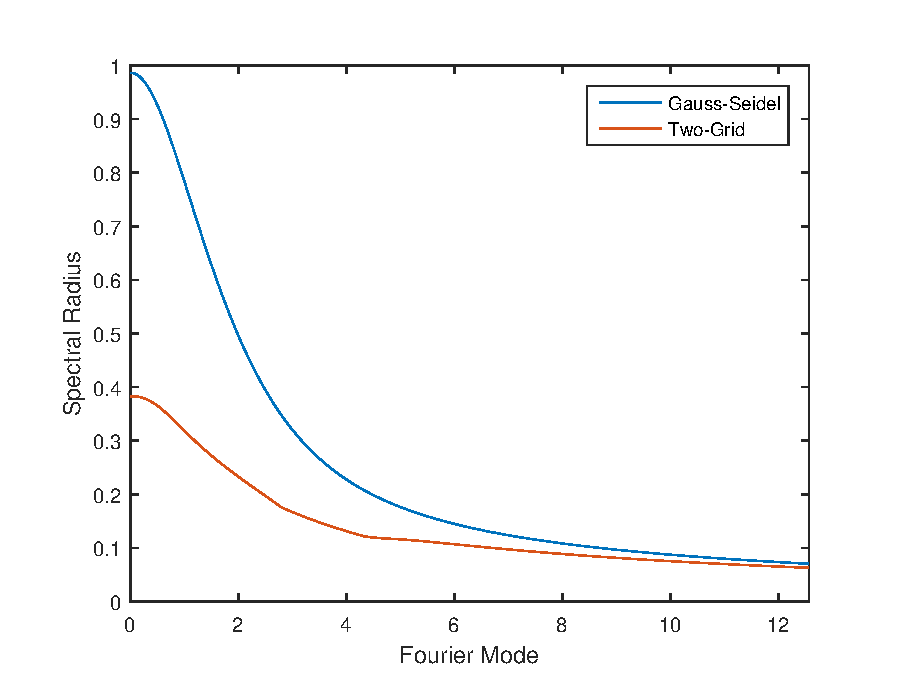
\includegraphics[width=\textwidth]{figures/P1_Fourier_69G.eps}
		\caption{}
	\end{subfigure}
\caption{The modal spectral radii for graphite with 69 group cross sections restricted to (a) $P_0$ scattering and (b) $P_1$ scattering.}
\label{fig::fourier_TG}
\end{figure}


\begin{table}
\label{tab::TG_counts}
\caption{Reduction of thermal iteration counts with two-grid acceleration for both a homogeneous graphit block as well as a graphite block with an air duct. 99 group cross sections are used with P1 scattering.}
\centering
\begin{tabular}{|c|c|c|}
\hline
Materials & Unaccelerated Iterations & Accelerated Iterations  \\
\hline \hline
Graphite Only & 2027 & 21 \\ \hline
Graphite + Air Duct & 2138 & 23 \\ \hline
\end{tabular}
\end{table}

%%%%%%%%%%%%%%%%%%%%%%%%%%%%%%%%%%%%%%%%%%%%%%%%%%%%%%%%%%%%%%%%%%%%%%
%%%%%%%%%%%%%%%%%%%%%%%%%%%%%%%%%%%%%%%%%%%%%%%%%%%%%%%%%%%%%%%%%%%%%%
\section{Ongoing Work}
\label{sec::OW}

Thus far, we have presented the overall objectives of the dissertation work and the work that has been completed to this point. There are still several areas of work that need to be completed. They are confined to two distinct areas: 1) remaining theoretical implementation and analysis of the polygonal finite element basis functions and their extension to the quadratic serendipity space and 2) scaling performance of MIP DSA in PDT.



%%%%%%%%%%%%%%%%%%%%%%%%%%%%%%%%%%%%%%%%%%%%%%%%%%%%%%%%%%%%%%%%%%%%%%
%%%%%%%%%%%%%%%%%%%%%%%%%%%%%%%%%%%%%%%%%%%%%%%%%%%%%%%%%%%%%%%%%%%%%%
\section{Expected Results and Summary}
\label{sec::ER}

We have presented the dissertation work that has been completed to date as well as the outline for all remaining work. We now quickly summarize the main topical areas of the dissertation project:

\begin{enumerate}
	\item Analyze the 2D linear polygonal basis functions for use in DGFEM transport calculations
	\item Perform the same analysis with the quadratic serendipity basis functions
	\item Determine the effects of numerical integration on highly-distorted polygonal elements
	\item Perform analysis on benchmark cases using polygonal meshes (including AMR)
	\item Analyze the 2D polygonal basis functions with DSA preconditioning through Fourier/numerical analysis
	\item Analyze the effects of AMR with polygonal basis functions on the MIP DSA PCG iteration counts (with and without bootstrapping)
	\item Extend the analysis of MIP DSA to arbitrary convex 3D polyhedra
	\item Implement MIP DSA in PDT using HYPRE
	\begin{itemize}
		\item Analyze the scalability of the method to high processor counts.
		\item Perform parametric studies on aggregation/partitioning factors to generate a performance model.
		\item Implement and perform analysis of two-grid acceleration at scale.
		\item Conclude with real-worl numerical experiments on high-fidelity meshes (IM1 and reactor geometries).
	\end{itemize}
\end{enumerate}

%%%%%%%%%%%%%%%%%%%%%%%%%%%%%%%%%%%%%%%%%%%%%%%%%%%%%%%%%%%%%%%%%%%%%%
%%%%%%%%%%%%%%%%%%%%%%%%%%%%%%%%%%%%%%%%%%%%%%%%%%%%%%%%%%%%%%%%%%%%%%
% References
\bibliographystyle{ans}
\bibliography{references}

\end{document}


